% =============================================================================
% RAPPORT DE STAGE — DROPPY
% Détection intelligente de fuites d'eau
% Style graphique : Noir & Bleu
% Compatible Overleaf / pdfLaTeX
% =============================================================================

\documentclass[12pt,a4paper,twoside]{report}

% =============================================================================
% ENCODAGE, LANGUE ET POLICES
% =============================================================================

\usepackage[utf8]{inputenc}
\usepackage[T1]{fontenc}
\usepackage[french]{babel}
\usepackage{lmodern}
\usepackage{microtype}

% =============================================================================
% MISE EN PAGE
% =============================================================================

\usepackage[
    top=2.7cm,
    bottom=2.7cm,
    left=3cm,
    right=2.5cm,
    headheight=18pt,
    headsep=0.45cm,
    footskip=1.1cm
]{geometry}

\usepackage{setspace}
\onehalfspacing

\setlength{\parindent}{0pt}
\setlength{\parskip}{6pt}

% =============================================================================
% COULEURS — IDENTITÉ DROPPY
% =============================================================================

\usepackage{xcolor}
\usepackage{amssymb}

\definecolor{DroppyBlue}{HTML}{1565C0}
\definecolor{DroppyLightBlue}{HTML}{EAF3FF}
\definecolor{DroppyDark}{HTML}{17202A}
\definecolor{DroppyGray}{HTML}{5F6B76}
\definecolor{DroppyLightGray}{HTML}{F4F6F8}
\definecolor{DroppyBorder}{HTML}{D9E2EC}

% =============================================================================
% TITRES
% =============================================================================

\usepackage{titlesec}
\usepackage{titletoc}

% -----------------------------------------------------------------------------
% Lignes décoratives
% -----------------------------------------------------------------------------

\newcommand{\chapterrule}{%
    \vspace{8pt}%
    \color{DroppyBlue}%
    \titlerule[1.2pt]%
}

\newcommand{\sectionrule}{%
    \vspace{3pt}%
    \color{DroppyBlue}%
    \titlerule[0.7pt]%
}

% -----------------------------------------------------------------------------
% Chapitres numérotés
% -----------------------------------------------------------------------------

\titleformat{\chapter}[display]
    {\normalfont\bfseries\color{DroppyDark}}
    {%
        \filleft
        \fontsize{14}{16}\selectfont
        \color{DroppyBlue}
        \MakeUppercase{\chaptertitlename}\ \thechapter
    }
    {10pt}
    {%
        \filleft
        \fontsize{28}{32}\selectfont
    }
    [\chapterrule]

\titlespacing*{\chapter}
    {0pt}
    {-10pt}
    {28pt}

% -----------------------------------------------------------------------------
% Chapitres non numérotés
% -----------------------------------------------------------------------------

\titleformat{name=\chapter,numberless}[display]
    {\normalfont\bfseries\color{DroppyDark}}
    {}
    {0pt}
    {\fontsize{25}{30}\selectfont}
    [\chapterrule]

% -----------------------------------------------------------------------------
% Sections
% -----------------------------------------------------------------------------

\titleformat{\section}
    {\normalfont\Large\bfseries\color{DroppyDark}}
    {\color{DroppyBlue}\thesection}
    {0.8em}
    {}
    [\sectionrule]

\titlespacing*{\section}
    {0pt}
    {22pt}
    {10pt}

% -----------------------------------------------------------------------------
% Sous-sections
% -----------------------------------------------------------------------------

\titleformat{\subsection}
    {\normalfont\large\bfseries\color{DroppyDark}}
    {\color{DroppyBlue}\thesubsection}
    {0.7em}
    {}

\titlespacing*{\subsection}
    {0pt}
    {15pt}
    {6pt}

% -----------------------------------------------------------------------------
% Sous-sous-sections
% -----------------------------------------------------------------------------

\titleformat{\subsubsection}
    {\normalfont\normalsize\bfseries\color{DroppyGray}}
    {\thesubsubsection}
    {0.6em}
    {}

\titlespacing*{\subsubsection}
    {0pt}
    {10pt}
    {4pt}

% =============================================================================
% FIGURES ET TABLEAUX
% =============================================================================

\usepackage{graphicx}
\usepackage{float}
\usepackage{booktabs}
\usepackage{array}
\usepackage{longtable}
\usepackage{tabularx}
\usepackage{multirow}
\usepackage{caption}
\usepackage{subcaption}
\usepackage{makecell}

% -----------------------------------------------------------------------------
% Style des légendes
% -----------------------------------------------------------------------------

\captionsetup{
    font=small,
    labelfont={bf,color=DroppyBlue},
    textfont={color=DroppyGray},
    labelsep=period,
    skip=8pt
}

% =============================================================================
% LISTES
% =============================================================================

\usepackage{enumitem}

\setlist[itemize]{
    leftmargin=1.5cm,
    itemsep=3pt,
    topsep=5pt,
    label=\textcolor{DroppyBlue}{\small$\blacktriangleright$}
}

\setlist[enumerate]{
    leftmargin=1.5cm,
    itemsep=4pt,
    topsep=5pt
}

% =============================================================================
% TABLEAUX
% =============================================================================

\newcolumntype{Y}{>{\raggedright\arraybackslash}X}

% =============================================================================
% CODE SOURCE
% =============================================================================

\usepackage{listings}

\definecolor{codegreen}{HTML}{2E7D32}
\definecolor{codegray}{HTML}{6B7280}
\definecolor{codepurple}{HTML}{7B1FA2}
\definecolor{backcolour}{HTML}{F5F7FA}
\definecolor{codeblue}{HTML}{1565C0}

\lstdefinestyle{pfe}{
    backgroundcolor=\color{backcolour},
    commentstyle=\color{codegreen},
    keywordstyle=\color{codeblue}\bfseries,
    numberstyle=\tiny\color{codegray},
    stringstyle=\color{codepurple},
    basicstyle=\ttfamily\footnotesize,
    breakatwhitespace=false,
    breaklines=true,
    captionpos=b,
    keepspaces=true,
    numbers=left,
    numbersep=8pt,
    showspaces=false,
    showstringspaces=false,
    showtabs=false,
    tabsize=2,
    frame=single,
    framerule=0.5pt,
    rulecolor=\color{DroppyBorder},
    xleftmargin=8pt,
    framexleftmargin=8pt,
    extendedchars=true,
    literate={é}{{\'e}}1 {è}{{\`e}}1 {ê}{{\^e}}1 {ë}{{\"e}}1
             {à}{{\`a}}1 {â}{{\^a}}1 {ä}{{\"a}}1 {ç}{{\c c}}1
             {î}{{\^i}}1 {ï}{{\"i}}1 {ô}{{\^o}}1 {ö}{{\"o}}1
             {ù}{{\`u}}1 {û}{{\^u}}1 {ü}{{\"u}}1 {œ}{{\oe}}1
             {É}{{\'E}}1 {È}{{\`E}}1 {Ê}{{\^E}}1 {À}{{\`A}}1
             {Â}{{\^A}}1 {Ç}{{\c C}}1 {Î}{{\^I}}1 {Ô}{{\^O}}1
}

\lstset{style=pfe}

% =============================================================================
% ENCADRÉS
% =============================================================================

\usepackage[most]{tcolorbox}

\newtcolorbox{droppybox}[1][]{
    enhanced,
    breakable,
    colback=DroppyLightBlue,
    colframe=DroppyBlue,
    boxrule=0.6pt,
    arc=2mm,
    left=8pt,
    right=8pt,
    top=7pt,
    bottom=7pt,
    #1
}

% =============================================================================
% LIENS
% =============================================================================

\usepackage{hyperref}

\hypersetup{
    colorlinks=true,
    linkcolor=DroppyBlue,
    citecolor=DroppyBlue,
    urlcolor=DroppyBlue,
    filecolor=DroppyBlue,
    pdftitle={Rapport de Stage — Droppy},
    pdfauthor={Aydi Ala},
    pdfsubject={
        Détection intelligente de fuites d'eau par IoT et intelligence artificielle
    },
    pdfcreator={LaTeX}
}

% =============================================================================
% COMMANDES PERSONNALISÉES
% =============================================================================

\newcommand{\droppy}{
    \textbf{\textcolor{DroppyBlue}{Droppy}}
}

\newcommand{\tech}[1]{
    \textbf{\textcolor{DroppyBlue}{#1}}
}

% =============================================================================
% MACRO POUR LES FIGURES UML
% =============================================================================

\newcommand{\umlfigure}[2]{%
    \begin{figure}[H]
        \centering

        \IfFileExists{images/#1.pdf}{%
            \includegraphics[width=\textwidth]{images/#1.pdf}%
        }{%
            \IfFileExists{images/#1.png}{%
                \includegraphics[width=\textwidth]{images/#1.png}%
            }{%
                \begin{droppybox}
                    \centering
                    \textbf{Diagramme : #2}\\[0.4cm]

                    \small
                    Fichier \texttt{\detokenize{images/#1.png}} non trouvé.\\[0.2cm]

                    Générez-le depuis
                    \texttt{\detokenize{diagrams/#1.puml}}
                    avec PlantUML.
                \end{droppybox}%
            }%
        }

        \caption{#2}
        \label{fig:#1}

    \end{figure}%
}

% =============================================================================
% PIED DE PAGE — NUMÉRO UNIQUEMENT
% =============================================================================

\usepackage{fancyhdr}

\pagestyle{fancy}

% Supprimer complètement le contenu de l'en-tête et du pied de page
\fancyhf{}

% Aucun élément dans l'en-tête
\renewcommand{\headrulewidth}{0pt}

% Numéro de page uniquement, centré et en bleu
\fancyfoot[C]{%
    \small
    \bfseries
    \color{DroppyBlue}
    \thepage
}

% Pas de ligne dans le pied de page
\renewcommand{\footrulewidth}{0pt}

% =============================================================================
% STYLE DES PAGES DE CHAPITRE
% =============================================================================
%
% La classe report utilise le style "plain" sur la première page
% de chaque chapitre. On applique exactement le même style :
% numéro de page centré et bleu.
% =============================================================================

\fancypagestyle{plain}{
    \fancyhf{}

    \fancyfoot[C]{%
        \small
        \bfseries
        \color{DroppyBlue}
        \thepage
    }

    \renewcommand{\headrulewidth}{0pt}
    \renewcommand{\footrulewidth}{0pt}
}

% =============================================================================
% TABLE DES MATIÈRES
% =============================================================================

\usepackage{tocloft}

\renewcommand{\cftchapfont}{
    \bfseries
    \color{DroppyDark}
}

\renewcommand{\cftchappagefont}{
    \bfseries
    \color{DroppyBlue}
}

\renewcommand{\cftsecfont}{
    \color{DroppyGray}
}

\renewcommand{\cftsecpagefont}{
    \color{DroppyDark}
}

\setlength{\cftbeforechapskip}{10pt}
\setlength{\cftbeforesecskip}{3pt}

\renewcommand{\cftchapleader}{
    \cftdotfill{\cftdotsep}
}

% =============================================================================
% DÉBUT DU DOCUMENT
% =============================================================================

\begin{document}

% =============================================================================
% PAGE DE GARDE
% =============================================================================

\begin{titlepage}

\thispagestyle{empty}

\begin{center}

\vspace*{0.3cm}

{\Large\bfseries
RÉPUBLIQUE TUNISIENNE
}

\vspace{0.25cm}

{\large\bfseries
UNIVERSITÉ PRIVÉE DE TUNISIE
}

\vspace{0.7cm}


\includegraphics[
    width=4.7cm
]{images/logo_iteams_uni_vecto__1_-removebg-preview.png}

\vspace{0.7cm}

{\color{DroppyBlue}\rule{13.5cm}{1.2pt}}

\vspace{0.45cm}

{
    \fontsize{24}{29}\selectfont
    \bfseries
    \color{DroppyDark}
    Rapport de Stage d'Été
}

\vspace{0.45cm}

{\color{DroppyBlue}\rule{13.5cm}{0.5pt}}

\vspace{0.7cm}

{
    \Large
    \bfseries
    \color{DroppyDark}

    Développement d'une plateforme intelligente\\
    de détection de fuites d'eau basée sur l'IoT\\
    et l'intelligence artificielle
}

\vspace{0.7cm}

\begin{droppybox}

\centering

{
    \large
    \bfseries
    Application Droppy
}

\vspace{0.2cm}

{
    \normalsize
    \textit{Water Leak Detection \& Anomaly Analysis Suite}
}

\end{droppybox}

\vspace{1.0cm}

\begin{tabular}{
    >{\bfseries}r
    @{\hspace{0.5cm}}
    l
}

\textcolor{DroppyBlue}{Entreprise d'accueil :}
&
SFM Connect -- Groupe SFM, Tunis
\\[0.35cm]

\textcolor{DroppyBlue}{Élaboré par :}
&
Aydi \textsc{Ala}
\\[0.35cm]

\textcolor{DroppyBlue}{Encadrant professionnel :}
&
Mr. Fadi \textsc{Bouricha}

\end{tabular}

\vfill

{\color{DroppyBlue}\rule{13.5cm}{0.5pt}}

\vspace{0.35cm}

{
    \large
    \bfseries
    Année universitaire : 2025 / 2026
}

\end{center}

\end{titlepage}

% =============================================================================
% REMERCIEMENTS
% =============================================================================

\chapter*{Remerciements}

\addcontentsline{toc}{chapter}{Remerciements}

Je tiens à exprimer ma profonde gratitude à l'équipe de
\textbf{SFM Connect}, branche du Groupe SFM, pour m'avoir accueilli
et accompagné tout au long de ce stage.

Cette expérience m'a permis de mettre en pratique mes connaissances
et de développer de nouvelles compétences dans les domaines du
développement logiciel, de l'IoT et de l'intelligence artificielle.

Je remercie tout particulièrement
\textbf{Mr. Fadi Bouricha}, mon encadrant professionnel, pour son
accompagnement, ses conseils, sa disponibilité et la confiance
accordée tout au long de la réalisation de ce projet.

Mes remerciements s'adressent également à l'ensemble des membres de
l'équipe pour leur disponibilité, leurs conseils techniques et les
échanges qui ont contribué à enrichir mon expérience professionnelle.

Enfin, j'adresse mes sincères remerciements à mes enseignants ainsi
qu'à ma famille et à mes proches pour leur soutien et leurs
encouragements durant cette période.

% =============================================================================
% RÉSUMÉ
% =============================================================================

\chapter*{Résumé}

\addcontentsline{toc}{chapter}{Résumé}

Ce rapport présente la conception et la réalisation de
\textbf{Droppy}, une suite logicielle multi-services destinée à la
détection automatique de fuites d'eau et d'anomalies dans les réseaux
de distribution.

Développée au sein de SFM Connect, la solution combine des données
issues de capteurs IoT, des règles métier hydrauliques telles que le
\textit{Minimum Night Flow} et la détection d'incohérences entre
l'état des vannes et le débit, ainsi que des méthodes d'apprentissage
automatique, notamment \textbf{Isolation Forest} et un modèle de
prévision de consommation.

L'architecture repose sur trois composants principaux : un
microservice dédié à l'intelligence artificielle développé avec
Python et FastAPI, un backend d'intégration développé avec Spring Boot
et intégrant des notifications en temps réel, ainsi qu'un tableau de
bord web développé avec Angular~19.

La solution vise ainsi à proposer une supervision intelligente capable
d'exploiter les données de télémétrie, d'identifier des comportements
inhabituels et de fournir aux opérateurs des informations exploitables
pour faciliter la détection et le suivi des anomalies.

\textbf{\textcolor{DroppyBlue}{Mots-clés :}}
IoT, fuite d'eau, intelligence artificielle, Isolation Forest,
FastAPI, Spring Boot, Angular, Minimum Night Flow, détection
d'anomalies.

% =============================================================================
% ABSTRACT
% =============================================================================

\chapter*{Abstract}

\addcontentsline{toc}{chapter}{Abstract}

This report presents the design and implementation of
\textbf{Droppy}, a multi-service software suite dedicated to automatic
water leak and anomaly detection in distribution networks.

Developed at SFM Connect, the solution combines data collected from
IoT sensors, hydraulic business rules such as the
\textit{Minimum Night Flow} and valve-flow inconsistency detection,
together with machine learning techniques including
\textbf{Isolation Forest} and a consumption forecasting model.

The architecture is based on three main components: an artificial
intelligence microservice developed with Python and FastAPI, an
integration backend developed with Spring Boot and supporting
real-time notifications, and a web dashboard developed with Angular~19.

The proposed solution aims to provide intelligent supervision capable
of processing telemetry data, identifying unusual behaviors, and
providing operators with actionable information to facilitate anomaly
detection and monitoring.

\textbf{\textcolor{DroppyBlue}{Keywords:}}
IoT, water leak, artificial intelligence, Isolation Forest, FastAPI,
Spring Boot, Angular, Minimum Night Flow, anomaly detection.

\clearpage

% =============================================================================
% TABLE DES MATIÈRES
% =============================================================================

\tableofcontents

\clearpage

% =============================================================================
% LISTE DES FIGURES
% =============================================================================

\listoffigures

\addcontentsline{toc}{chapter}{Liste des figures}

\clearpage

% =============================================================================
% LISTE DES TABLEAUX
% =============================================================================

\listoftables

\addcontentsline{toc}{chapter}{Liste des tableaux}

\clearpage

% =============================================================================
% CHAPITRES
% =============================================================================
%
% IMPORTANT :
%
% Le numéro du chapitre dépend de l'ordre des \chapter{} présents
% dans les fichiers inclus et non du nom du fichier.
%
% Les noms de fichiers existants sont conservés ici.
% =============================================================================

% -----------------------------------------------------------------------------
% CHAPITRE 1
% -----------------------------------------------------------------------------

% =============================================================================
% CHAPITRE 1 — INTRODUCTION GÉNÉRALE
% =============================================================================

\chapter{Introduction générale}

% =============================================================================
% 1.1 CONTEXTE GÉNÉRAL
% =============================================================================

\section{Contexte général}

L'eau constitue une ressource naturelle essentielle au développement des sociétés
et au fonctionnement de nombreuses activités humaines. Sa gestion efficace
représente aujourd'hui un enjeu majeur, particulièrement dans les régions
confrontées à des périodes de stress hydrique et à une augmentation constante
des besoins en consommation. Dans ce contexte, la réduction des pertes d'eau
et l'amélioration de la surveillance des installations hydrauliques constituent
des problématiques importantes pour les entreprises, les collectivités et les
gestionnaires d'infrastructures.

Les réseaux de distribution et les installations hydrauliques peuvent être
affectés par différents types de dysfonctionnements, notamment les fuites,
les consommations inhabituelles, les variations anormales de débit ou encore
les problèmes liés au fonctionnement des vannes. Lorsque ces événements ne
sont pas détectés rapidement, ils peuvent entraîner une consommation excessive
d'eau, une augmentation des coûts d'exploitation, des dégradations matérielles
et, dans certains cas, des conséquences environnementales importantes.

Les méthodes traditionnelles de surveillance reposent généralement sur des
contrôles périodiques et des inspections manuelles. Bien que ces approches
permettent d'identifier certains problèmes, elles présentent des limites
lorsqu'il s'agit de détecter rapidement des anomalies apparaissant entre deux
inspections. L'exploitation continue des données issues de capteurs connectés
constitue ainsi une approche permettant d'améliorer la surveillance des
installations et de réduire le délai de détection des événements anormaux.

L'intégration de l'Internet des Objets
(\textit{Internet of Things -- IoT}) permet justement de collecter en continu
des données provenant des équipements physiques. Ces données peuvent ensuite
être exploitées par des systèmes logiciels capables de les analyser
automatiquement et d'assister les opérateurs dans la supervision des
installations.

% =============================================================================
% 1.2 PRÉSENTATION DE L'ENTREPRISE ET DU PROJET
% =============================================================================

\section{Présentation de l'entreprise et du projet}

C'est dans ce contexte que s'inscrit le présent projet, réalisé au sein de
\textbf{SFM Connect}, branche spécialisée dans les solutions liées à
l'Internet des Objets (\textit{Internet of Things -- IoT}) du
\textbf{Groupe SFM}, à Tunis.

SFM Connect développe des solutions permettant de connecter des équipements
physiques à des plateformes numériques afin de collecter, traiter et exploiter
leurs données. Dans le domaine de la gestion de l'eau, le projet
\textbf{Droppy} s'inscrit dans cette démarche en proposant une solution
destinée à améliorer la supervision des installations hydrauliques à partir
des données provenant de capteurs IoT.

Ces capteurs transmettent régulièrement différentes informations relatives au
fonctionnement du réseau, notamment le débit d'eau
(\texttt{flow\_rate}), la consommation cumulative
(\texttt{consumption}) ainsi que l'état d'une vanne
(\texttt{state}), généralement représenté par les états
\texttt{ON} et \texttt{OFF}. Chaque équipement est identifié de manière
unique, notamment à travers son adresse MAC, permettant ainsi d'associer les
différentes mesures au capteur correspondant.

L'exploitation de ces données permet de passer d'une simple collecte
d'informations à une véritable approche de supervision intelligente. Le
système développé dans le cadre de ce projet vise ainsi à analyser
automatiquement les données de télémétrie afin d'identifier des comportements
inhabituels pouvant correspondre à des fuites ou à d'autres anomalies de
fonctionnement.

% =============================================================================
% 1.3 PRÉSENTATION DE LA SOLUTION DROPPY
% =============================================================================

\section{Présentation de la solution Droppy}

Le projet \textbf{Droppy -- Water Leak Detection \& Anomaly Analysis Suite}
consiste en la conception et la réalisation d'une plateforme logicielle
intelligente dédiée à la détection des fuites d'eau et à l'analyse des
anomalies provenant des capteurs IoT.

La solution adopte une architecture distribuée organisée autour de plusieurs
composants spécialisés. Elle associe une interface web développée avec
\textbf{Angular 19}, un backend principal développé avec
\textbf{Spring Boot 3} et un service dédié aux traitements d'intelligence
artificielle développé avec \textbf{FastAPI} et Python.

Cette organisation permet de séparer les différentes responsabilités du
système. Le backend constitue le service central de la plateforme et assure
notamment l'intégration des données, l'orchestration des traitements, la
gestion de la persistance ainsi que la communication avec l'interface
utilisateur. Le service d'intelligence artificielle prend en charge les
traitements nécessaires à l'analyse des données et à la détection des
comportements inhabituels.

Le tableau de bord constitue l'interface principale de supervision. Il permet
aux utilisateurs de consulter les informations relatives aux capteurs,
d'analyser les données historiques, de visualiser les anomalies détectées et
de recevoir des notifications lorsqu'un événement important est identifié.

Les choix techniques ainsi que l'organisation détaillée de cette architecture
seront présentés dans les chapitres consacrés à l'analyse des besoins et à la
conception de la solution.

% =============================================================================
% 1.4 PROBLÉMATIQUE
% =============================================================================

\section{Problématique}

La principale difficulté d'un système de surveillance des installations
hydrauliques réside dans la capacité à distinguer un comportement normal
d'un comportement réellement anormal. Une augmentation du débit peut, par
exemple, correspondre à une utilisation normale de l'installation, mais elle
peut également être le signe d'une fuite. De la même manière, un état
particulier de la vanne associé à un débit inattendu peut révéler une
incohérence dans le fonctionnement du système.

L'analyse d'un seul indicateur ne permet donc pas toujours d'obtenir une
détection suffisamment fiable. Il devient nécessaire de prendre en
considération plusieurs signaux provenant des capteurs et d'étudier leur
évolution dans le temps.

Par ailleurs, les règles statiques peuvent être efficaces pour identifier
certains cas connus, mais elles présentent des limites face à des
comportements inhabituels qui n'ont pas été explicitement définis à l'avance.
L'utilisation de techniques d'intelligence artificielle et d'apprentissage
automatique permet alors de compléter les règles métier en recherchant
automatiquement des comportements atypiques dans les données.

La problématique principale de ce projet peut ainsi être formulée comme suit :

\begin{quote}
\textit{
Comment concevoir et mettre en œuvre une plateforme intelligente, fiable
et évolutive permettant d'exploiter les données issues de capteurs IoT afin
de détecter automatiquement les fuites d'eau et les anomalies de
fonctionnement, tout en fournissant aux opérateurs une interface de
supervision capable de présenter les résultats et de générer des alertes
en temps réel ?
}
\end{quote}

% =============================================================================
% 1.5 APPROCHE PROPOSÉE
% =============================================================================

\section{Approche proposée}

Afin de répondre à cette problématique, le projet adopte une approche hybride
combinant des méthodes déterministes et des techniques d'apprentissage
automatique.

Dans un premier temps, les données provenant des capteurs sont nettoyées et
prétraitées afin de traiter les valeurs incohérentes et de préparer les
données pour les différentes étapes d'analyse. Une attention particulière est
accordée à l'exploitation des mesures de débit et de consommation en tant que
séries temporelles.

Dans un deuxième temps, des règles métier sont appliquées afin d'identifier
certaines situations particulières. Parmi ces mécanismes figure notamment
l'analyse du \textit{Minimum Night Flow} (MNF), permettant d'étudier les
consommations observées pendant les périodes nocturnes, ainsi que la détection
d'incohérences entre l'état d'une vanne et les mesures de débit.

En complément de ces règles, le système intègre des méthodes d'apprentissage
automatique. L'algorithme \textbf{Isolation Forest}, utilisé dans une approche
de détection non supervisée, permet d'identifier des observations présentant
un comportement inhabituel par rapport aux données observées.

Un mécanisme de prévision de la consommation est également utilisé afin de
comparer les tendances attendues aux comportements réellement observés.

Cette combinaison permet ainsi de dépasser les limites d'une détection
reposant uniquement sur des seuils fixes. Les résultats des différents
mécanismes d'analyse peuvent ensuite être exploités par le système de
supervision afin d'informer les opérateurs et de faciliter l'identification
des situations nécessitant une intervention.

% =============================================================================
% 1.6 ARCHITECTURE GÉNÉRALE DE LA SOLUTION
% =============================================================================

\section{Architecture générale de la solution}

L'architecture générale de Droppy repose sur trois composants principaux qui
collaborent pour assurer la collecte, le traitement, l'analyse et la
visualisation des données.

Le premier composant correspond au \textbf{frontend Angular 19}. Il constitue
l'interface utilisateur de la plateforme et permet notamment d'afficher les
informations relatives aux capteurs, les anomalies détectées, les données
historiques ainsi que différentes visualisations graphiques. Il permet
également de recevoir des événements en temps réel.

Le deuxième composant est le \textbf{backend Spring Boot 3}, qui constitue
le service central de l'application. Il assure l'intégration des différents
traitements, la gestion des données, la persistance des informations et la
communication avec l'interface utilisateur.

Le troisième composant correspond au \textbf{service d'intelligence
artificielle FastAPI}. Il regroupe les traitements liés à la préparation des
données, à la détection des anomalies et à la prévision. Il communique avec
le backend à travers des API afin de fournir les résultats nécessaires à la
plateforme.

Cette organisation permet de séparer clairement les responsabilités entre
l'interface utilisateur, la logique applicative et les traitements
d'intelligence artificielle. Elle facilite ainsi la maintenance du système
et permet d'envisager son évolution vers de nouveaux types de capteurs, de
nouvelles méthodes d'analyse ou de nouvelles fonctionnalités.

L'architecture détaillée, les flux de communication entre les composants
ainsi que les choix technologiques seront présentés dans les chapitres
consacrés à la conception de la solution.

% =============================================================================
% 1.7 OBJECTIFS DU PROJET
% =============================================================================

\section{Objectifs du projet}

L'objectif général de ce projet est de concevoir et développer une plateforme
intelligente permettant d'améliorer la détection des fuites d'eau et la
supervision des installations hydrauliques à partir de données IoT.

Plus précisément, les objectifs poursuivis sont les suivants :

\begin{itemize}

    \item Mettre en place un pipeline permettant de charger, nettoyer et
    prétraiter les données de télémétrie issues des capteurs IoT ;

    \item Développer des mécanismes de détection basés sur des règles métier
    afin d'identifier les comportements anormaux liés notamment au débit,
    à la consommation et à l'état des vannes ;

    \item Intégrer des méthodes d'apprentissage automatique, notamment
    l'algorithme \textbf{Isolation Forest}, afin de détecter automatiquement
    des comportements atypiques ;

    \item Mettre en place un mécanisme de prévision de la consommation
    permettant d'analyser les tendances et d'identifier d'éventuels écarts
    par rapport au comportement attendu ;

    \item Développer un service d'intelligence artificielle avec
    \textbf{FastAPI} afin d'exposer les fonctionnalités d'analyse,
    de prédiction et de prévision à travers des API REST ;

    \item Développer un backend central avec \textbf{Spring Boot 3}
    permettant d'assurer l'intégration des différents composants de la
    plateforme ;

    \item Mettre en œuvre un système de notifications en temps réel afin
    d'informer rapidement les opérateurs lorsqu'une anomalie importante
    est détectée ;

    \item Concevoir un tableau de bord interactif avec
    \textbf{Angular 19} permettant aux utilisateurs de visualiser les
    données, les anomalies et les informations relatives aux capteurs ;

    \item Assurer la persistance et la gestion structurée des données afin
    de permettre la consultation et l'analyse des historiques ;

    \item Mettre en place des tests permettant de vérifier le bon
    fonctionnement des différents composants de la solution.

\end{itemize}

% =============================================================================
% 1.8 MÉTHODOLOGIE ET ORGANISATION DU PROJET
% =============================================================================

\section{Méthodologie et organisation du projet}

La réalisation du projet a été organisée autour de plusieurs étapes
successives permettant de progresser progressivement de l'analyse du besoin
jusqu'à la validation de la solution.

La première étape a consisté à comprendre le fonctionnement du système IoT
et la structure des données provenant des capteurs. Cette phase a permis
d'identifier les différentes variables disponibles et de déterminer les
informations nécessaires à la détection des anomalies.

La deuxième étape a concerné le traitement et la préparation des données.
Les données brutes ont été analysées, nettoyées et transformées afin de
constituer une base exploitable pour les différents mécanismes de détection.

La troisième étape a consisté à concevoir et développer les mécanismes
d'analyse en combinant les règles métier et les méthodes d'apprentissage
automatique. Cette phase a notamment permis d'intégrer la détection des
comportements atypiques ainsi que les mécanismes de prévision de la
consommation.

La quatrième étape a été consacrée au développement de l'architecture
applicative. Les différents services ont été mis en place afin d'assurer
la communication entre les composants de la plateforme. En parallèle,
l'interface de supervision a été développée afin de permettre la
visualisation et l'exploitation des résultats.

Enfin, une phase de tests et de validation a permis de vérifier le
comportement des différentes composantes du système et d'évaluer la
cohérence des résultats produits.

% =============================================================================
% 1.9 STRUCTURE DU RAPPORT
% =============================================================================

\section{Structure du rapport}

Afin de présenter de manière progressive les différentes étapes de réalisation
du projet, ce rapport est organisé en plusieurs chapitres complémentaires.

Le premier chapitre présente le contexte général du projet, l'entreprise
d'accueil, la solution Droppy, la problématique ainsi que les objectifs
poursuivis.

Le deuxième chapitre est consacré à l'analyse des besoins et au cahier des
charges. Il présente notamment les acteurs du système, les besoins
fonctionnels et non fonctionnels, les contraintes ainsi que les critères
permettant d'évaluer la réussite de la solution.

Les chapitres suivants présentent progressivement l'analyse de l'existant,
la conception de la solution, l'architecture logicielle, les modèles UML
ainsi que les choix technologiques adoptés.

Une partie du rapport est ensuite consacrée à la réalisation de la plateforme.
Elle présente les principales fonctionnalités développées au niveau du
backend, du service d'intelligence artificielle et de l'interface de
supervision.

Les mécanismes d'intelligence artificielle et de détection des anomalies
sont également détaillés, notamment le prétraitement des données, les règles
métier, l'algorithme \textbf{Isolation Forest} ainsi que les mécanismes de
prévision.

Enfin, le rapport présente la stratégie de tests et de validation mise en
place afin d'évaluer le fonctionnement de la solution, avant de terminer
par une conclusion générale présentant les principales contributions
réalisées, les limites identifiées et les perspectives d'évolution de
la plateforme.

% =============================================================================
% CONCLUSION DU CHAPITRE
% =============================================================================

\section*{Conclusion du chapitre}

\addcontentsline{toc}{section}{Conclusion du chapitre}

Ce premier chapitre a permis de présenter le contexte général dans lequel
s'inscrit le projet \textbf{Droppy}, ainsi que les enjeux liés à la
surveillance intelligente des installations hydrauliques. L'analyse du
problème a mis en évidence les limites des approches traditionnelles et la
nécessité de disposer d'une solution capable d'exploiter en continu les
données issues des capteurs IoT.

La solution proposée repose sur une approche combinant traitement des
données, règles métier et techniques d'apprentissage automatique afin
d'améliorer la détection des comportements anormaux. L'architecture retenue
permet également de séparer les différentes responsabilités du système et
de fournir une interface de supervision adaptée aux besoins des utilisateurs.

Après avoir défini le contexte, la problématique et les objectifs du projet,
le chapitre suivant sera consacré à l'analyse détaillée des besoins et à
l'élaboration du cahier des charges. Cette étape permettra de transformer
les objectifs identifiés en exigences fonctionnelles et non fonctionnelles
précises, constituant ainsi la base de la conception de la solution.

% -----------------------------------------------------------------------------
% CHAPITRE 2
% -----------------------------------------------------------------------------

% =============================================================================
% CHAPITRE 2 — ANALYSE DES BESOINS ET CAHIER DES CHARGES
% =============================================================================

\chapter{Analyse des besoins et cahier des charges}

% =============================================================================
% 2.1 INTRODUCTION
% =============================================================================

\section{Introduction}

Après avoir présenté dans le chapitre précédent le contexte général du
projet Droppy, sa problématique ainsi que les objectifs poursuivis, ce
chapitre est consacré à l'analyse des besoins et à la définition du cahier
des charges de la solution.

L'objectif de cette phase est de traduire le problème métier en exigences
concrètes permettant de guider la conception et la réalisation de la
plateforme. Il s'agit notamment d'identifier les utilisateurs concernés,
les sources de données, les fonctionnalités attendues ainsi que les
contraintes techniques et qualitatives auxquelles le système doit répondre.

L'analyse commence par une étude du domaine de la gestion des réseaux d'eau
et des problématiques liées aux fuites et aux comportements anormaux. Une
étude de l'existant permet ensuite de mettre en évidence les limites des
approches traditionnelles et de justifier la nécessité d'une supervision
plus automatisée et intelligente.

La vision fonctionnelle de Droppy est ensuite présentée afin de décrire la
chaîne globale allant de la collecte des données jusqu'à leur analyse et à
leur restitution à l'opérateur.

Enfin, les acteurs du système, les besoins fonctionnels, les besoins non
fonctionnels, les contraintes du projet ainsi que les critères de réussite
sont définis afin de constituer le cahier des charges de la solution.

% =============================================================================
% 2.2 COMPRÉHENSION DU DOMAINE MÉTIER
% =============================================================================

\section{Compréhension du domaine métier}

\subsection{Enjeux de la gestion des réseaux d'eau}

La gestion efficace d'un réseau de distribution d'eau nécessite une
surveillance régulière des différents équipements et des flux de
consommation. Le gestionnaire doit être capable de suivre l'évolution des
débits, des consommations ainsi que l'état des équipements afin
d'identifier rapidement toute situation inhabituelle.

Dans un réseau instrumenté, les capteurs permettent de transformer les
équipements physiques en sources de données exploitables par une plateforme
logicielle. La surveillance ne repose alors plus uniquement sur des
inspections ponctuelles, mais peut s'appuyer sur une observation continue
du comportement du réseau.

Cette évolution présente un intérêt particulier dans le contexte de la
détection des fuites. Une fuite non détectée peut entraîner une perte
importante d'eau et provoquer des coûts supplémentaires pour l'exploitant.
La rapidité de détection constitue donc un élément essentiel de la
supervision.

\subsection{Typologie des anomalies}

Dans le cadre du projet Droppy, une anomalie correspond à un comportement
qui s'écarte du fonctionnement habituellement observé.

Plusieurs situations peuvent notamment être considérées :

\begin{itemize}

    \item une augmentation inhabituelle du débit ;

    \item une consommation anormalement élevée pendant une période de faible
    activité ;

    \item une consommation nocturne inhabituelle ;

    \item une incohérence entre l'état d'une vanne et le débit observé ;

    \item une évolution inhabituelle d'une série temporelle ;

    \item un comportement globalement atypique détecté automatiquement par
    un modèle d'apprentissage automatique.

\end{itemize}

Il est important de souligner qu'une anomalie ne correspond pas
nécessairement à une fuite. Elle constitue plutôt un signal nécessitant
une analyse complémentaire. La plateforme doit donc fournir suffisamment
d'informations pour permettre à l'opérateur d'interpréter le comportement
détecté.

\subsection{Données disponibles et télémétrie IoT}

Les capteurs IoT constituent la principale source de données de Droppy.

Les informations exploitées peuvent notamment comprendre :

\begin{itemize}

    \item le débit d'eau ;

    \item la consommation ;

    \item l'état d'une vanne ;

    \item l'identifiant du dispositif ;

    \item l'horodatage associé à la mesure.

\end{itemize}

Chaque équipement doit pouvoir être identifié de manière unique afin de
maintenir la correspondance entre les mesures reçues et leur source.

La dimension temporelle des données constitue également un élément
important. L'analyse d'une mesure isolée étant généralement insuffisante,
le système doit pouvoir exploiter l'évolution des données au cours du
temps.

\subsection{Enjeux de la détection précoce}

La détection précoce représente un enjeu majeur pour la surveillance des
réseaux d'eau.

Une anomalie détectée rapidement permet à l'opérateur d'analyser la
situation et, lorsque cela est nécessaire, de déclencher une intervention
avant que le problème ne provoque des pertes importantes.

L'objectif de Droppy est donc de réduire autant que possible le délai entre
l'apparition d'un comportement inhabituel et son identification par
l'utilisateur.

Cette exigence justifie la mise en place d'une chaîne automatisée combinant
collecte des données, analyse, détection et notification.

% =============================================================================
% 2.3 ÉTUDE DE L'EXISTANT
% =============================================================================

\section{Étude de l'existant}

\subsection{Surveillance traditionnelle}

Les approches traditionnelles de surveillance des réseaux d'eau reposent
principalement sur les inspections périodiques, les relevés manuels et
l'utilisation de seuils définis à l'avance.

Dans ce contexte, l'opérateur consulte les mesures disponibles et recherche
des valeurs pouvant indiquer un dysfonctionnement.

Cette approche reste pertinente pour certains scénarios, mais elle devient
plus difficile à maintenir lorsque le nombre d'équipements et la fréquence
des mesures augmentent.

\subsection{Approches basées sur les seuils}

Une méthode courante consiste à définir un seuil à partir duquel une alerte
est déclenchée.

Par exemple, une règle peut considérer qu'un débit dépassant une certaine
valeur constitue une situation potentiellement anormale.

Cependant, le comportement normal d'un équipement peut varier selon
l'heure, le jour, la période d'utilisation ou les caractéristiques du site.
Un seuil fixe ne permet donc pas toujours de représenter correctement
l'ensemble des situations possibles.

\subsection{Limites identifiées}

Plusieurs limites peuvent ainsi être identifiées.

Premièrement, les inspections manuelles ne garantissent pas une détection
immédiate des anomalies.

Deuxièmement, les seuils statiques peuvent générer des faux positifs lorsque
la variation observée correspond à un fonctionnement normal.

Troisièmement, certaines anomalies peuvent rester invisibles lorsqu'elles
ne dépassent pas les seuils prédéfinis.

Enfin, l'analyse manuelle devient difficile lorsque plusieurs capteurs
produisent continuellement des données.

Ces limites montrent qu'une approche automatisée est nécessaire afin
d'exploiter efficacement les volumes de données disponibles.

\subsection{Besoin d'une supervision intelligente}

Une supervision intelligente doit être capable de combiner plusieurs
sources d'information et plusieurs mécanismes d'analyse.

Dans Droppy, cette approche repose sur une combinaison entre des règles
métier et des techniques d'apprentissage automatique.

Les règles métier permettent d'identifier des situations connues, tandis
que les modèles d'apprentissage automatique permettent de rechercher des
comportements atypiques dans les données.

Cette complémentarité permet d'obtenir une analyse plus riche qu'une
approche reposant uniquement sur des seuils fixes.

% =============================================================================
% 2.4 VISION FONCTIONNELLE DE DROPPY
% =============================================================================

\section{Vision fonctionnelle de Droppy}

\subsection{Vision globale}

Droppy est conçu comme une plateforme de supervision intelligente permettant
de transformer les données brutes provenant des équipements IoT en
informations exploitables par les opérateurs.

La solution est organisée autour de trois composants logiciels principaux :

\begin{itemize}

    \item \textbf{Angular 19}, utilisé pour développer le tableau de bord
    de supervision ;

    \item \textbf{Spring Boot 3}, utilisé comme service backend central pour
    l'intégration, l'orchestration et la gestion des événements ;

    \item \textbf{FastAPI et Python}, utilisés pour les traitements de
    données et les mécanismes d'intelligence artificielle.

\end{itemize}

Le dépôt du projet confirme cette organisation en distinguant notamment
le frontend \texttt{dashboard-angular}, le service backend
\texttt{core-service} et le moteur d'intelligence artificielle situé dans
le répertoire \texttt{src}. :contentReference[oaicite:3]{index=3}

\subsection{Chaîne globale de traitement}

Le fonctionnement fonctionnel de Droppy peut être représenté comme une
chaîne composée des étapes suivantes :

\begin{enumerate}

    \item collecte des données provenant des équipements IoT ;

    \item ingestion des données par le système ;

    \item nettoyage et préparation des données ;

    \item application des règles métier ;

    \item analyse par les modèles d'apprentissage automatique ;

    \item génération des résultats de détection ou de prévision ;

    \item enregistrement des informations importantes ;

    \item transmission des événements au tableau de bord ;

    \item consultation et interprétation des résultats par l'opérateur.

\end{enumerate}

Cette chaîne permet de transformer progressivement une donnée brute en une
information pouvant être utilisée pour la supervision et la prise de
décision.

\subsection{Valeur ajoutée de la solution}

La valeur ajoutée de Droppy réside principalement dans l'intégration de
plusieurs mécanismes au sein d'une même plateforme.

La solution ne se limite pas à afficher les mesures provenant des capteurs.
Elle permet également de les nettoyer, de les analyser et d'identifier
automatiquement certains comportements inhabituels.

L'utilisation d'un modèle tel que \textbf{Isolation Forest} permet notamment
de rechercher des observations atypiques sans dépendre exclusivement de
seuils prédéfinis.

La plateforme intègre également des mécanismes de prévision ainsi que des
notifications permettant de transmettre rapidement les événements
importants à l'utilisateur.

Le dépôt du projet indique notamment l'existence des fonctionnalités de
réentraînement des modèles, de prédiction combinée et de prévision de
consommation. :contentReference[oaicite:4]{index=4}

\subsection{Résultats attendus}

À partir des données collectées, le système doit permettre d'obtenir
plusieurs types de résultats :

\begin{itemize}

    \item identification de comportements atypiques ;

    \item détection de situations pouvant correspondre à des fuites ;

    \item production de prévisions de consommation ;

    \item génération d'événements d'alerte ;

    \item visualisation des résultats dans le tableau de bord ;

    \item conservation des informations nécessaires à l'analyse historique.

\end{itemize}

L'objectif final est de fournir à l'opérateur une information synthétique
et exploitable plutôt qu'un simple ensemble de mesures brutes.

% =============================================================================
% 2.5 IDENTIFICATION DES ACTEURS
% =============================================================================

\section{Identification des acteurs}

L'identification des acteurs permet de déterminer les différentes entités
participant au fonctionnement de la solution et leurs responsabilités.

Contrairement à une application classique, Droppy implique à la fois des
utilisateurs humains, des équipements physiques et des services logiciels.

\subsection{Opérateur / gestionnaire}

L'opérateur constitue l'utilisateur principal de la plateforme.

Il utilise le tableau de bord pour :

\begin{itemize}

    \item consulter les équipements ;

    \item visualiser les données de télémétrie ;

    \item suivre les anomalies détectées ;

    \item consulter les historiques ;

    \item recevoir les notifications ;

    \item analyser les tendances de consommation.

\end{itemize}

Son rôle est principalement orienté vers la supervision et l'interprétation
des résultats fournis par le système.

\subsection{Capteurs et équipements IoT}

Les équipements IoT représentent les sources physiques des données.

Ils transmettent les mesures nécessaires au fonctionnement de la chaîne
d'analyse. Ces données peuvent notamment concerner le débit, la
consommation et l'état des vannes.

Les équipements doivent être identifiables afin de permettre au système
d'associer chaque mesure au dispositif correspondant.

\subsection{Backend applicatif}

Le backend Spring Boot joue le rôle de service central d'intégration.

Il assure notamment :

\begin{itemize}

    \item la réception et l'intégration des données ;

    \item l'orchestration des traitements ;

    \item la communication avec le service d'intelligence artificielle ;

    \item la persistance des informations ;

    \item le routage des événements vers le tableau de bord.

\end{itemize}

Le dépôt indique notamment l'utilisation de Spring Boot 3, de mécanismes de
planification et de WebSockets pour les notifications en temps réel. :contentReference[oaicite:5]{index=5}

\subsection{Service d'intelligence artificielle}

Le microservice FastAPI constitue le moteur d'analyse de Droppy.

Il prend en charge les traitements liés aux données et à l'intelligence
artificielle, notamment :

\begin{itemize}

    \item le nettoyage des données ;

    \item le prétraitement ;

    \item l'application de certaines règles métier ;

    \item la détection des anomalies ;

    \item la prévision de consommation ;

    \item le réentraînement des modèles.

\end{itemize}

Le projet expose notamment des opérations de réentraînement, de prédiction
et de prévision pour un équipement donné. :contentReference[oaicite:6]{index=6}

\subsection{Interface de supervision}

L'interface Angular constitue le point d'accès principal de l'opérateur.

Elle permet de centraliser les résultats produits par les différents
services et de les présenter sous une forme visuelle.

Le tableau de bord permet notamment d'afficher les anomalies, les données
historiques et les graphiques de télémétrie tout en recevant les
notifications en temps réel. :contentReference[oaicite:7]{index=7}

% =============================================================================
% 2.6 BESOINS FONCTIONNELS
% =============================================================================

\section{Besoins fonctionnels}

Les besoins fonctionnels définissent les services que la plateforme doit
fournir pour répondre aux objectifs identifiés.

\subsection{Gestion des équipements}

\textbf{BF01 -- Gestion des équipements}

Le système doit permettre d'identifier et de consulter les équipements
surveillés.

Chaque équipement doit pouvoir être associé à ses différentes mesures et
à son historique afin de faciliter le suivi individuel.

\subsection{Ingestion des télémétries}

\textbf{BF02 -- Collecte des données}

Le système doit permettre de recevoir et d'intégrer les données produites
par les équipements IoT.

Les données doivent être correctement associées à leur équipement et à
leur instant de mesure.

\subsection{Nettoyage et prétraitement}

\textbf{BF03 -- Prétraitement}

Le système doit être capable de nettoyer et de préparer les données avant
leur analyse.

Cette étape doit notamment permettre de traiter les valeurs manquantes,
les incohérences et les transformations nécessaires à l'exploitation des
séries temporelles.

\subsection{Détection des anomalies}

\textbf{BF04 -- Détection des anomalies}

La plateforme doit identifier automatiquement les comportements atypiques
présents dans les données de télémétrie.

Un modèle de type \textbf{Isolation Forest} est utilisé pour contribuer à
cette détection.

\subsection{Détection des fuites}

\textbf{BF05 -- Détection des fuites}

Le système doit permettre d'identifier les situations pouvant correspondre
à une fuite.

La détection peut s'appuyer sur plusieurs indicateurs tels que le débit,
la consommation, l'état des vannes et les comportements observés pendant
les périodes de faible activité.

\subsection{Prévision de consommation}

\textbf{BF06 -- Prévision}

La plateforme doit permettre de produire des prévisions de consommation
afin de comparer les valeurs observées avec les tendances attendues.

Cette fonctionnalité peut également contribuer à identifier des écarts
significatifs dans le comportement d'un équipement.

\subsection{Gestion des alertes}

\textbf{BF07 -- Alertes}

Lorsqu'une anomalie importante est identifiée, le système doit pouvoir
générer un événement destiné à l'opérateur.

Les événements critiques doivent pouvoir être transmis rapidement au
tableau de bord.

\subsection{Supervision en temps réel}

\textbf{BF08 -- Supervision}

Le système doit fournir une interface permettant à l'opérateur de suivre
les informations importantes relatives au réseau.

La plateforme doit notamment permettre de consulter les anomalies, les
graphiques, les équipements et les notifications.

\subsection{Historisation}

\textbf{BF09 -- Historique}

Le système doit conserver les informations nécessaires au suivi historique
des données et des anomalies.

L'historique permet notamment de comparer le comportement actuel d'un
équipement avec ses observations précédentes.

\subsection{Réentraînement des modèles}

\textbf{BF10 -- Gestion des modèles}

Le système doit permettre de réentraîner les modèles d'intelligence
artificielle pour un équipement donné lorsque cela est nécessaire.

Cette fonctionnalité permet d'adapter les modèles aux nouvelles données
disponibles.

% =============================================================================
% 2.7 BESOINS NON FONCTIONNELS
% =============================================================================

\section{Besoins non fonctionnels}

\subsection{Performance}

\textbf{BNF01 -- Performance}

La plateforme doit traiter les données avec un temps de réponse acceptable
afin de permettre une utilisation fluide du tableau de bord.

\subsection{Fiabilité}

\textbf{BNF02 -- Fiabilité}

Les données doivent être traitées de manière cohérente et les mécanismes
d'analyse doivent limiter les erreurs liées aux données incomplètes ou
incohérentes.

\subsection{Temps réel}

\textbf{BNF03 -- Temps réel}

Les événements importants doivent pouvoir être transmis rapidement à
l'interface de supervision.

L'utilisation des WebSockets permet au backend de transmettre des
notifications sans nécessiter une actualisation permanente de la page.

\subsection{Sécurité}

\textbf{BNF04 -- Sécurité}

Les communications entre les différents composants doivent être protégées
et les accès aux fonctionnalités sensibles doivent être contrôlés.

\subsection{Maintenabilité}

\textbf{BNF05 -- Maintenabilité}

La séparation entre frontend, backend et service d'intelligence artificielle
doit faciliter la maintenance et l'évolution du système.

\subsection{Évolutivité}

\textbf{BNF06 -- Évolutivité}

La solution doit pouvoir intégrer de nouveaux équipements, de nouvelles
méthodes d'analyse et de nouvelles fonctionnalités sans nécessiter une
refonte complète de l'architecture.

\subsection{Ergonomie}

\textbf{BNF07 -- Ergonomie}

Le tableau de bord doit présenter les informations de manière claire et
compréhensible afin de permettre à l'opérateur d'identifier rapidement
les situations nécessitant son attention.

% =============================================================================
% 2.8 CONTRAINTES DU PROJET
% =============================================================================

\section{Contraintes du projet}

La réalisation de Droppy doit respecter plusieurs contraintes techniques
et organisationnelles.

\subsection{Hétérogénéité technologique}

La solution repose sur plusieurs technologies et environnements :

\begin{itemize}

    \item Python et FastAPI pour le service d'intelligence artificielle ;

    \item Java et Spring Boot pour le backend ;

    \item TypeScript et Angular 19 pour le frontend ;

    \item outils de gestion de données et de modèles pour le pipeline IA.

\end{itemize}

Cette diversité nécessite une définition claire des interfaces entre les
différents composants.

\subsection{Nature temporelle des données}

Les données de télémétrie sont associées à des instants de mesure. Leur
ordre temporel doit donc être conservé afin de permettre l'analyse des
évolutions et des tendances.

\subsection{Communication inter-services}

Le backend doit assurer une communication fiable avec le service
d'intelligence artificielle et avec le frontend.

Le dépôt du projet indique notamment l'utilisation de HTTP/REST entre les
services ainsi que de WebSockets pour les notifications temps réel. :contentReference[oaicite:8]{index=8}

\subsection{Gestion de la persistance}

Les informations nécessaires au suivi des équipements, des événements et
des analyses doivent être correctement persistées.

Le projet utilise notamment Liquibase pour la gestion et le versionnement
des évolutions du schéma de base de données. :contentReference[oaicite:9]{index=9}

\subsection{Validation de la solution}

La solution doit être accompagnée de tests permettant de vérifier les
différents composants.

Le dépôt comprend notamment des tests dédiés au pipeline Python et aux
fonctionnalités de l'API, ainsi que des procédures de test pour les
différents composants de l'application. :contentReference[oaicite:10]{index=10}

% =============================================================================
% 2.9 CAHIER DES CHARGES FONCTIONNEL
% =============================================================================

\section{Cahier des charges fonctionnel}

Le cahier des charges fonctionnel synthétise les principales exigences
identifiées au cours de l'analyse.

\subsection{Tableau des exigences}

\begin{table}[H]
\centering
\caption{Synthèse des exigences fonctionnelles de Droppy}
\label{tab:exigences-droppy}

\renewcommand{\arraystretch}{1.35}

\begin{tabularx}{\textwidth}{
    >{\bfseries\centering\arraybackslash}p{1.5cm}
    >{\raggedright\arraybackslash}p{3.1cm}
    >{\raggedright\arraybackslash}X
    >{\centering\arraybackslash}p{1.8cm}
}

\toprule

ID & Fonctionnalité & Description & Priorité \\

\midrule

BF01 &
Gestion des équipements &
Identifier et consulter les équipements surveillés. &
Haute \\

BF02 &
Collecte des données &
Recevoir et intégrer les télémétries provenant des capteurs. &
Haute \\

BF03 &
Prétraitement &
Nettoyer et préparer les données avant leur analyse. &
Haute \\

BF04 &
Détection des anomalies &
Identifier automatiquement les comportements atypiques. &
Haute \\

BF05 &
Détection des fuites &
Identifier les situations pouvant correspondre à une fuite. &
Haute \\

BF06 &
Prévision &
Analyser les tendances et prévoir la consommation. &
Moyenne \\

BF07 &
Alertes &
Informer l'opérateur lorsqu'une anomalie importante est détectée. &
Haute \\

BF08 &
Supervision &
Visualiser les données, équipements et anomalies. &
Haute \\

BF09 &
Historique &
Permettre la consultation des données historiques. &
Moyenne \\

BF10 &
Gestion des modèles &
Permettre le réentraînement et l'exploitation des modèles. &
Moyenne \\

\bottomrule

\end{tabularx}

\end{table}

\subsection{Priorisation des exigences}

Les exigences ont été classées selon leur importance pour le fonctionnement
global de la solution.

Les fonctionnalités de priorité \textbf{haute} constituent le noyau de
Droppy. Elles comprennent notamment la collecte des données, le
prétraitement, la détection des anomalies, la détection des fuites, les
alertes et la supervision.

Les fonctionnalités de priorité \textbf{moyenne} viennent compléter le
système et permettent d'améliorer les capacités d'analyse et d'exploitation
des données.

Cette priorisation permet de concentrer les efforts de développement sur
les fonctionnalités essentielles avant d'intégrer les fonctionnalités
complémentaires.

% =============================================================================
% 2.10 CRITÈRES DE RÉUSSITE
% =============================================================================

\section{Critères de réussite}

La réussite de la plateforme Droppy est évaluée selon plusieurs dimensions.

\subsection{Critères fonctionnels}

Le système doit être capable :

\begin{itemize}

    \item de recevoir correctement les données de télémétrie ;

    \item de traiter et préparer les données ;

    \item d'identifier les comportements atypiques ;

    \item de détecter les situations pouvant correspondre à des fuites ;

    \item de produire des prévisions ;

    \item de générer et transmettre les alertes ;

    \item d'afficher les résultats dans le tableau de bord.

\end{itemize}

\subsection{Critères techniques}

La solution doit également respecter plusieurs critères techniques :

\begin{itemize}

    \item communication correcte entre les différents services ;

    \item fonctionnement des échanges temps réel ;

    \item persistance fiable des informations ;

    \item possibilité de réentraîner les modèles ;

    \item modularité des composants ;

    \item présence de mécanismes de test et de validation.

\end{itemize}

\subsection{Critères liés à l'utilisateur}

Enfin, le système doit permettre à l'opérateur :

\begin{itemize}

    \item d'accéder rapidement aux informations importantes ;

    \item d'identifier facilement les anomalies ;

    \item de consulter l'historique ;

    \item de comprendre les résultats produits ;

    \item de réagir rapidement lorsqu'une alerte critique est générée.

\end{itemize}

% =============================================================================
% 2.11 CONCLUSION
% =============================================================================

\section{Conclusion}

Ce chapitre a permis de transformer la problématique générale de la
détection des fuites d'eau en un ensemble d'exigences fonctionnelles et
non fonctionnelles concrètes.

L'analyse du domaine métier a montré l'importance de disposer d'une
surveillance continue capable d'exploiter les données issues des
équipements IoT. L'étude de l'existant a également mis en évidence les
limites des inspections périodiques et des approches reposant uniquement
sur des seuils fixes.

La vision fonctionnelle de Droppy repose ainsi sur une chaîne complète
allant de la collecte des télémétries jusqu'à leur analyse et leur
restitution dans une interface de supervision. Cette chaîne combine
traitement des données, règles métier, apprentissage automatique,
prévision et notifications.

Les acteurs du système ainsi que les besoins fonctionnels, les besoins non
fonctionnels et les contraintes ont ensuite été identifiés. Le cahier des
charges obtenu constitue la base de la phase de conception.

Le chapitre suivant sera consacré à la \textbf{conception de la solution}.
Il présentera l'architecture globale de Droppy, les interactions entre ses
différents composants, les flux de données ainsi que les modèles permettant
de formaliser la conception du système.

% -----------------------------------------------------------------------------
% CHAPITRE 3
% -----------------------------------------------------------------------------

% =============================================================================
% CHAPITRE 3 — CONCEPTION ET ARCHITECTURE DE LA SOLUTION DROPPY
% =============================================================================

\chapter{Conception et architecture de la solution Droppy}

% =============================================================================
% 3.1 INTRODUCTION
% =============================================================================

\section{Introduction}

Après l'analyse des besoins présentée dans le chapitre précédent, cette étape
consiste à concevoir la solution Droppy et à définir son architecture.

La conception est présentée à travers plusieurs vues complémentaires permettant
de représenter le système sous différents angles : fonctionnel, architectural,
dynamique, statique et physique.

Les modèles retenus sont le diagramme de cas d'utilisation, l'architecture
globale, deux diagrammes de séquence, le diagramme de classes et le diagramme
de déploiement.


% =============================================================================
% 3.2 ARCHITECTURE GLOBALE
% =============================================================================

\section{Architecture globale}

Droppy repose sur une architecture distribuée organisée autour de trois
composants principaux : une application web Angular 19, un Core Service
Spring Boot 3 et un microservice d'intelligence artificielle développé avec
FastAPI.

Le Core Service constitue le point central de communication entre l'interface
utilisateur, le service d'intelligence artificielle et la base de données.
L'application Angular communique avec Spring Boot à travers des API REST et
un canal WebSocket pour les notifications en temps réel. Spring Boot
communique quant à lui avec le microservice FastAPI pour les opérations de
détection et de prévision.

\begin{figure}[H]
    \centering
    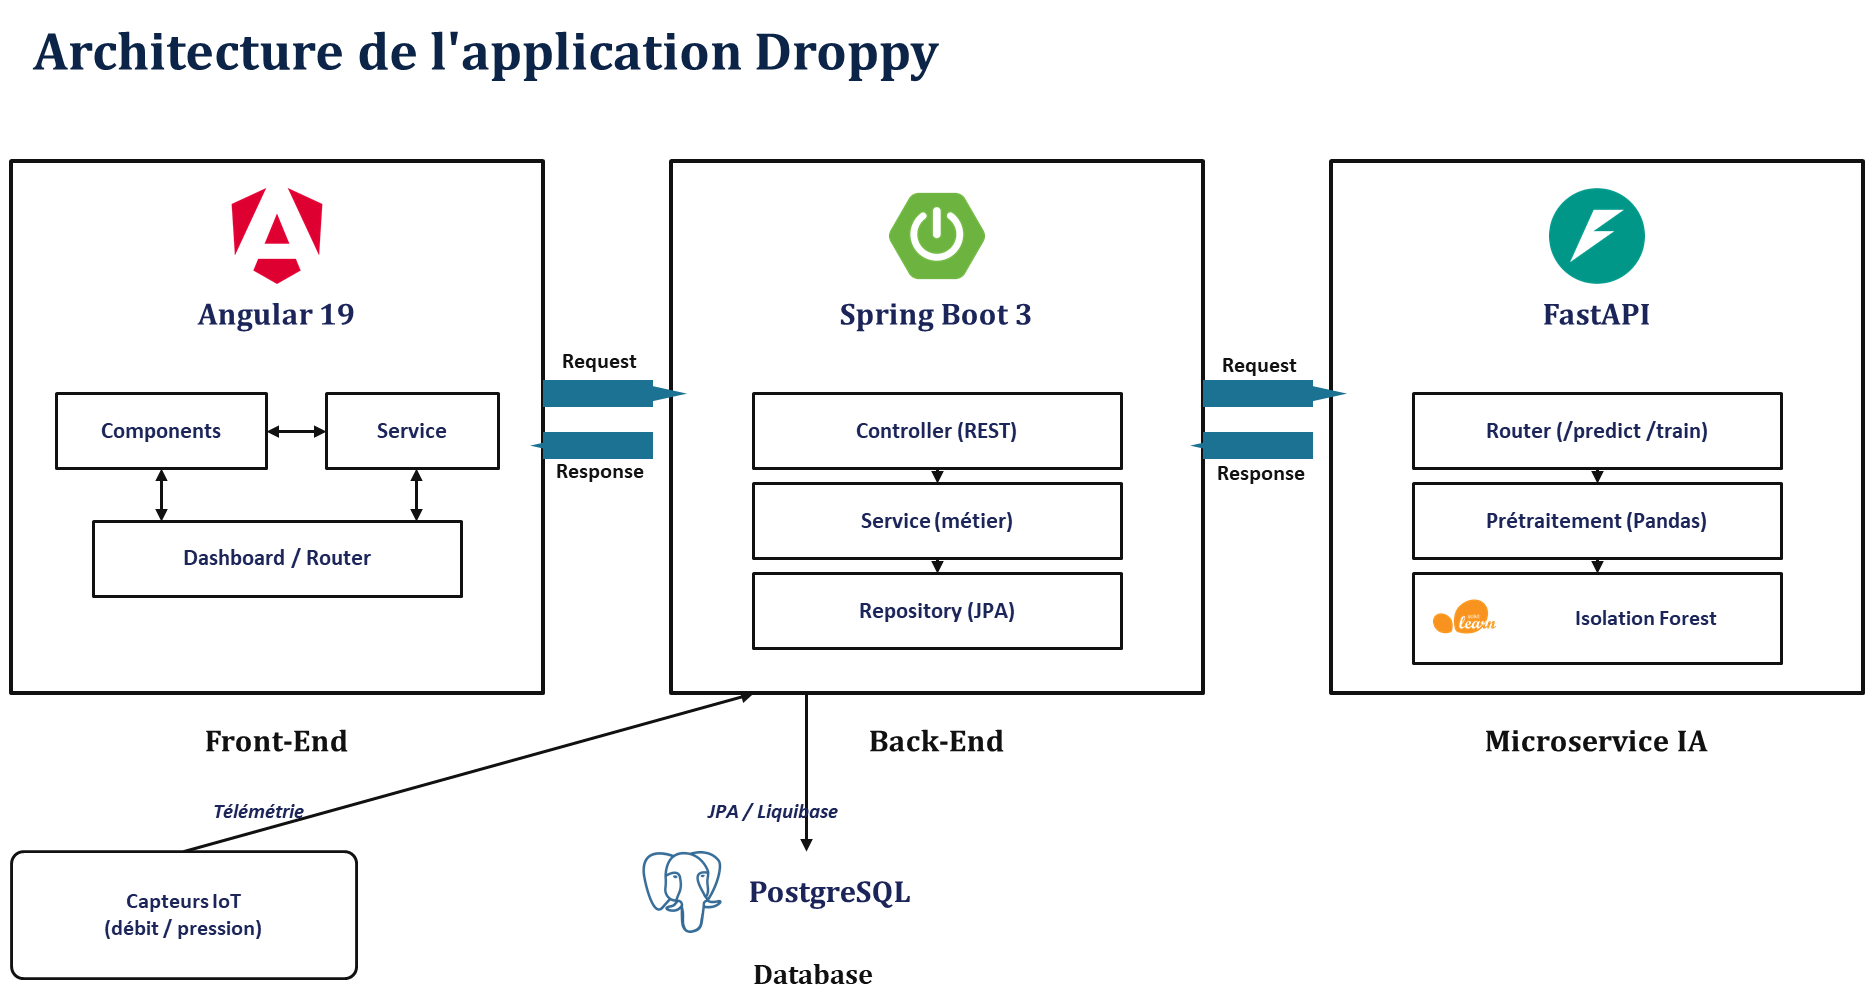
\includegraphics[width=0.95\textwidth]{images/architecture (2).png}
    \caption{Architecture globale de la solution Droppy}
    \label{fig:architecture-globale}
\end{figure}

Cette architecture permet de découpler l'interface, la logique métier et les
traitements d'intelligence artificielle, tout en conservant un point
d'orchestration central.


% =============================================================================
% 3.3 CAS D'UTILISATION
% =============================================================================

\section{Modélisation fonctionnelle}

Le diagramme de cas d'utilisation présente les principales interactions entre
l'utilisateur et la solution Droppy.

L'opérateur constitue l'acteur principal du système. Il utilise le dashboard
pour consulter les anomalies, visualiser les données, demander une analyse,
consulter les prévisions et traiter les anomalies détectées.

Les traitements automatiques sont également représentés afin de montrer que
certaines opérations, notamment l'analyse périodique des dispositifs, sont
déclenchées sans intervention directe de l'utilisateur.

\begin{figure}[H]
    \centering
    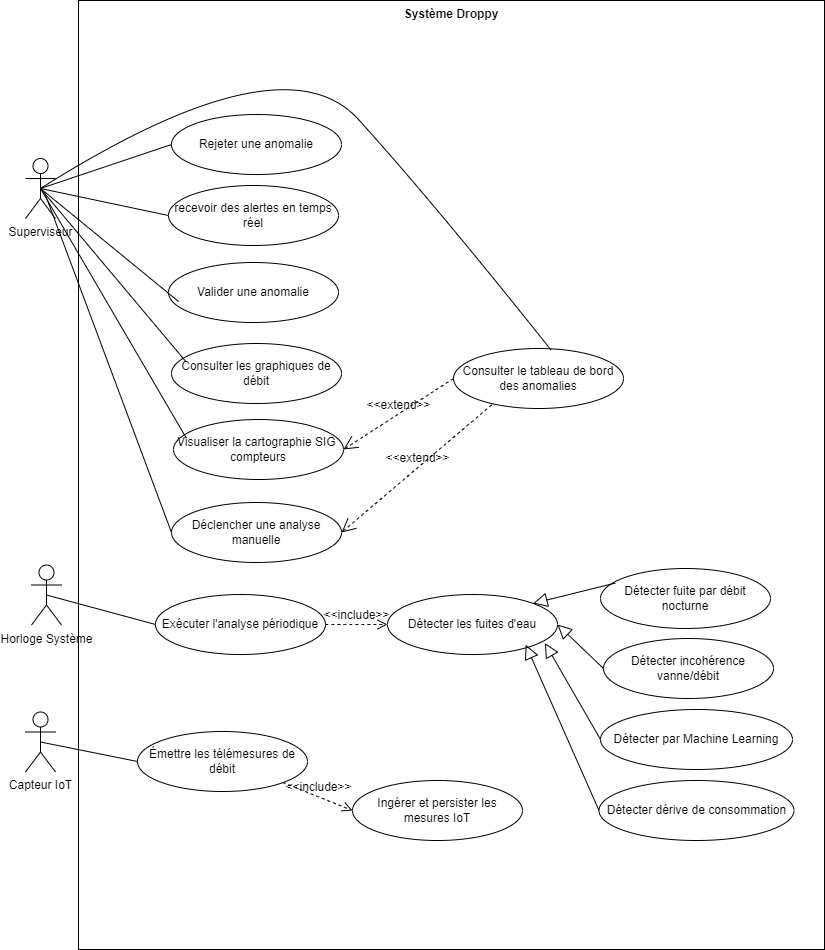
\includegraphics[width=\textwidth]{images/usecase.drawio.png}
    \caption{Diagramme de cas d'utilisation de Droppy}
    \label{fig:use-case-droppy}
\end{figure}

Ce modèle fournit ainsi une vue fonctionnelle synthétique des principales
interactions avec la plateforme.


% =============================================================================
% 3.4 MODELISATION DYNAMIQUE
% =============================================================================

\section{Modélisation dynamique}

Les diagrammes de séquence permettent de représenter les échanges entre les
différents composants lors de l'exécution des scénarios principaux de Droppy.

Deux scénarios ont été retenus : la détection d'une anomalie et la prévision
de consommation.


% -----------------------------------------------------------------------------
% 3.4.1 DETECTION
% -----------------------------------------------------------------------------

\subsection{Détection d'une anomalie}

Le premier scénario représente le processus de détection d'une anomalie.
L'analyse est déclenchée par le scheduler puis orchestrée par le Core Service,
qui sollicite le microservice FastAPI.

\begin{figure}[H]
    \centering
    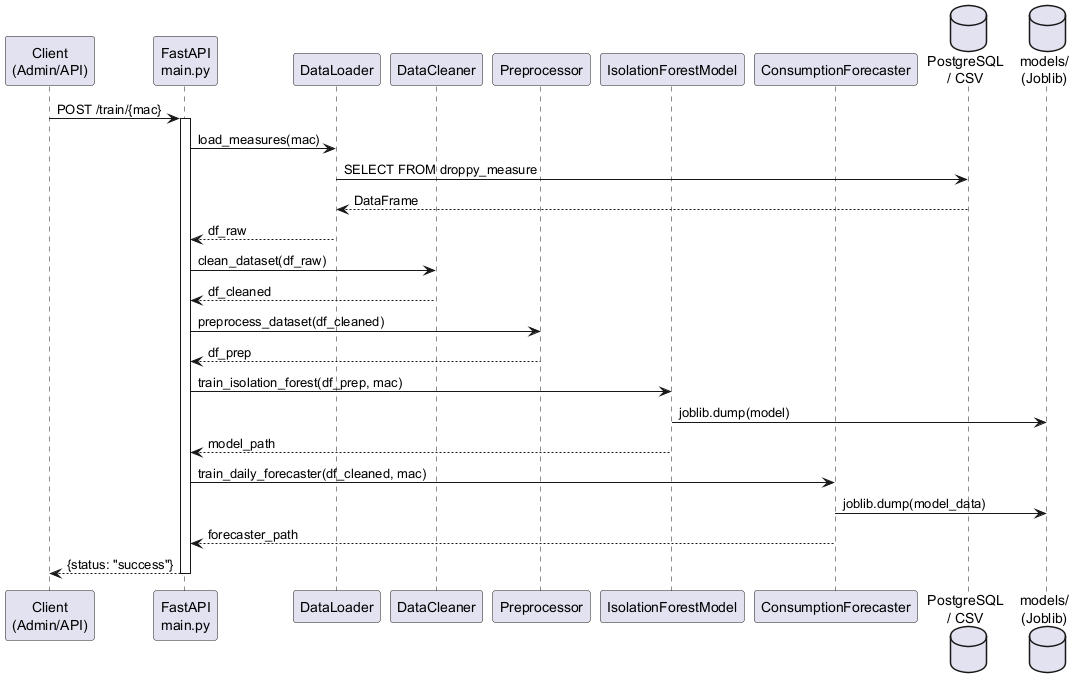
\includegraphics[width=\textwidth]{images/sequence_train.png}
    \caption{Séquence de détection d'une anomalie}
    \label{fig:sequence-detection}
\end{figure}

Le résultat retourné par le service IA est traité par Spring Boot avant
d'être enregistré et transmis au dashboard lorsque cela est nécessaire.


% -----------------------------------------------------------------------------
% 3.4.2 PREVISION
% -----------------------------------------------------------------------------

\subsection{Prévision de consommation}

Le second scénario décrit la demande d'une prévision depuis le dashboard.
La requête traverse le Core Service avant d'être transmise au microservice
FastAPI, qui exécute le modèle de prévision.

\begin{figure}[H]
    \centering
    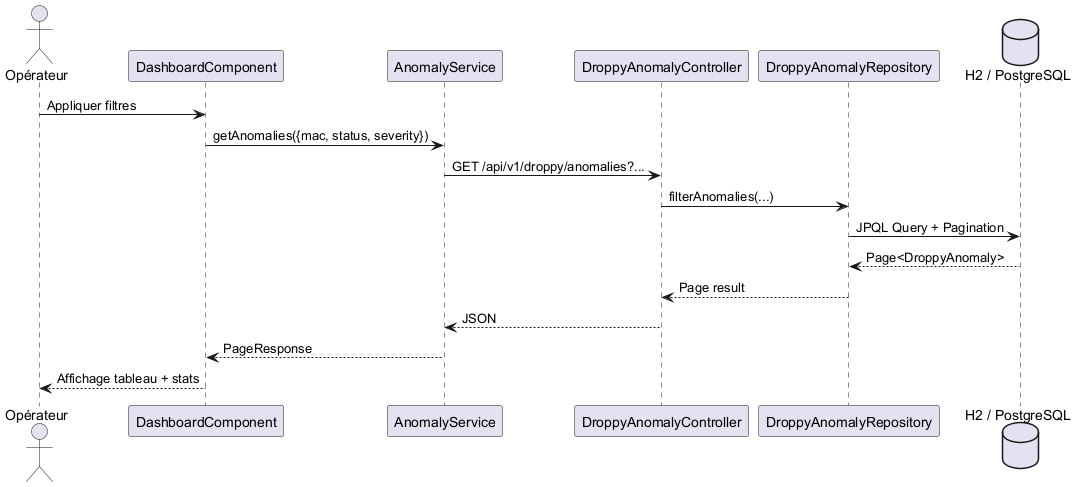
\includegraphics[width=\textwidth]{images/sequence_get.png}
    \caption{Séquence de prévision de consommation}
    \label{fig:sequence-prevision}
\end{figure}

Le résultat est ensuite retourné au dashboard afin d'être présenté à
l'opérateur sous une forme graphique.


% =============================================================================
% 3.5 DIAGRAMME DE CLASSES
% =============================================================================

\section{Modélisation statique}

Le diagramme de classes présente la structure des principaux éléments du
Core Service et leurs relations.

La conception suit une séparation des responsabilités entre les contrôleurs,
les services métier, les repositories et les entités persistantes. La classe
\texttt{DroppyAnomaly} constitue l'entité centrale pour la représentation et
le suivi des anomalies détectées.

\begin{figure}[H]
    \centering
    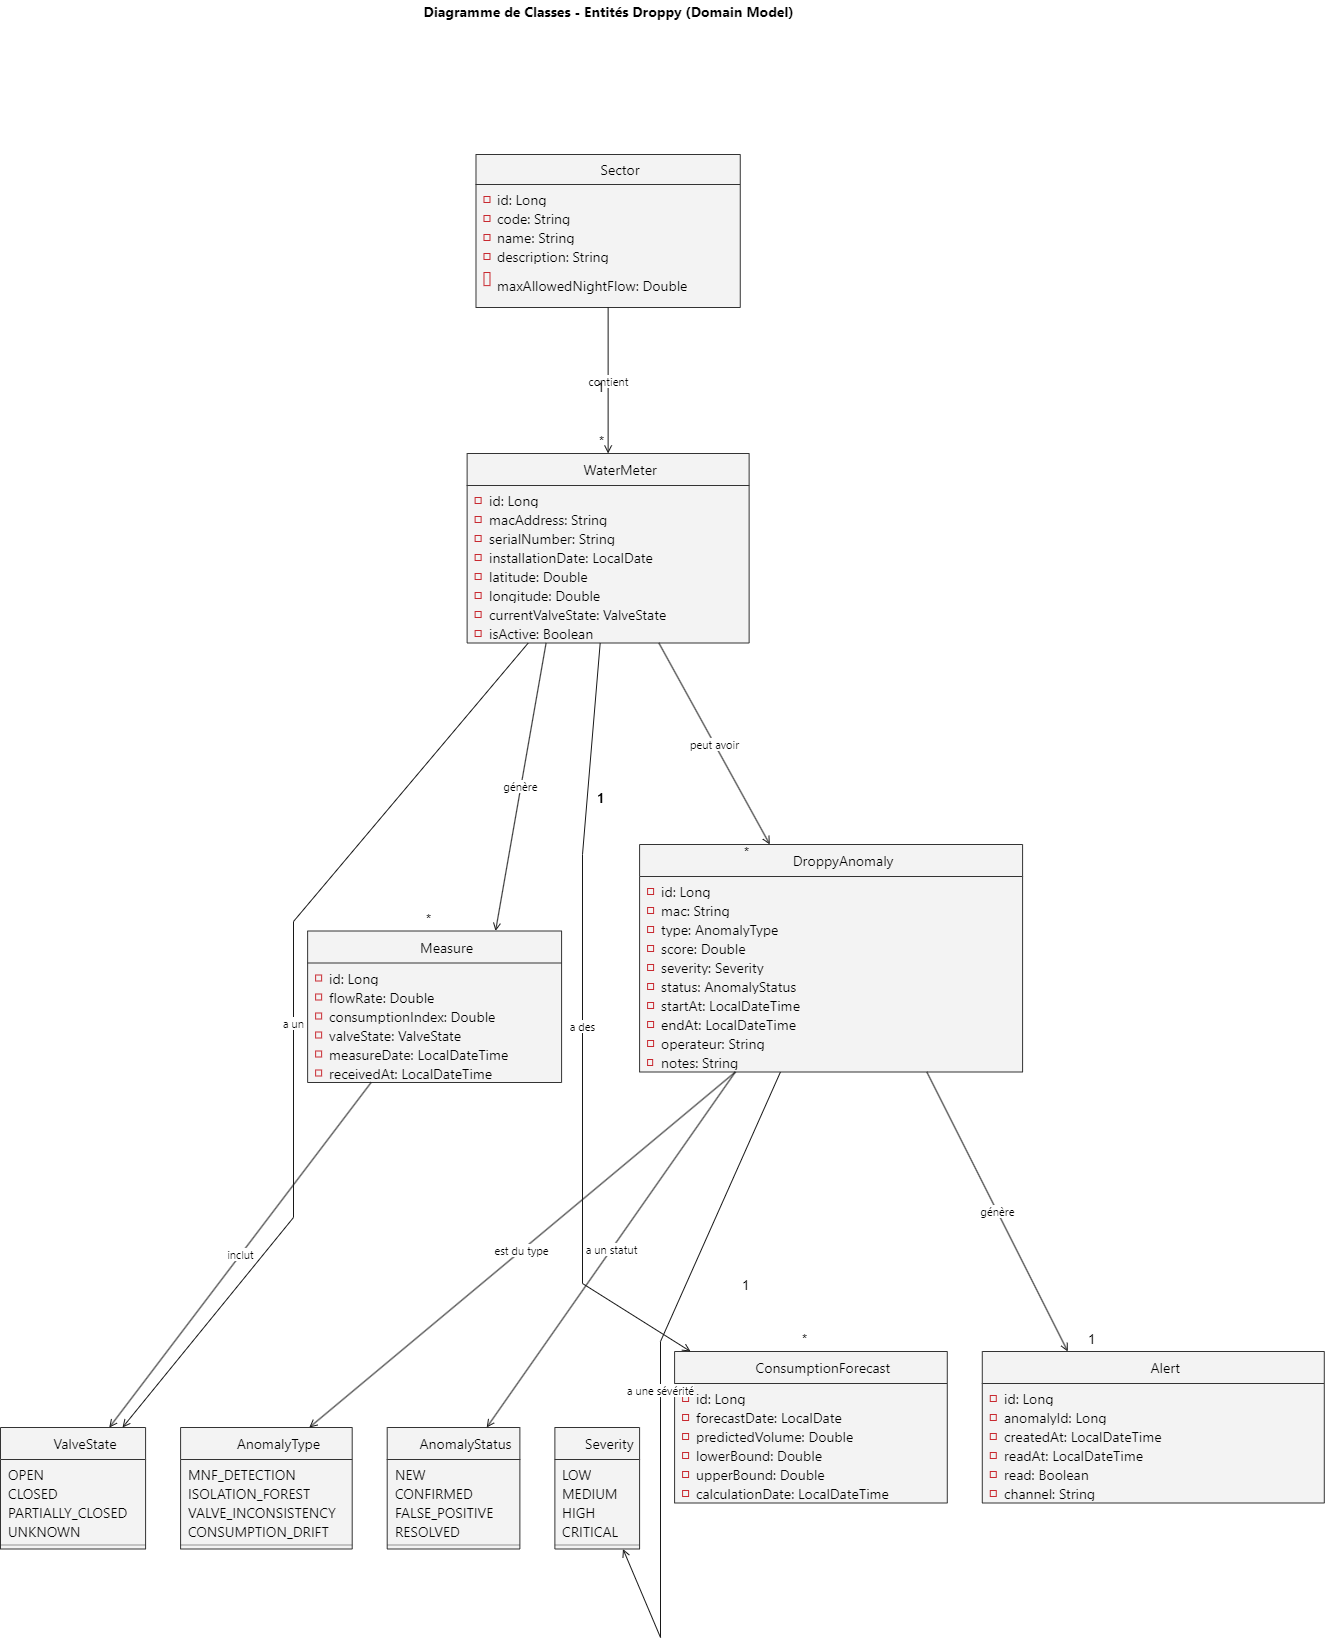
\includegraphics[width=\textwidth]{images/class.drawio.png}
    \caption{Diagramme de classes principal de Droppy}
    \label{fig:diagramme-classes}
\end{figure}

Cette organisation permet de maintenir une séparation claire entre
l'exposition des API, la logique métier et l'accès aux données.
\clearpage

% 
\section{Conclusion}

Ce chapitre a présenté la conception de Droppy à travers plusieurs vues
complémentaires.

L'architecture globale a permis de définir l'organisation des principaux
services, tandis que les diagrammes de cas d'utilisation et de séquence ont
permis de représenter les interactions et les scénarios essentiels. Le
diagramme de classes a décrit la structure statique du système et le diagramme
de déploiement a présenté son organisation dans l'environnement d'exécution.

Cette conception constitue la base de la réalisation technique présentée dans
le chapitre suivant.

% -----------------------------------------------------------------------------
% CHAPITRE 4
% -----------------------------------------------------------------------------

% =============================================================================
% CHAPITRE 4 — RÉALISATION ET PRÉSENTATION DE L'APPLICATION DROPPY
% =============================================================================

\chapter{Réalisation et présentation de l'application Droppy}

% =============================================================================
% 4.1 INTRODUCTION
% =============================================================================

\section{Introduction}

Après avoir présenté les besoins et la conception de la solution, ce chapitre
est consacré à la présentation de l'application Droppy réalisée.

L'objectif est de présenter les principales interfaces de la solution ainsi
que les fonctionnalités accessibles à travers le dashboard. Les différentes
captures d'écran permettent d'illustrer concrètement le résultat obtenu et
le parcours d'utilisation de l'application.


% =============================================================================
% 4.2 PRÉSENTATION GÉNÉRALE DE L'APPLICATION
% =============================================================================

\section{Présentation générale de l'application}

\subsection{Écran principal}

L'écran principal constitue le point d'entrée de l'application. Il offre une
vue synthétique des informations importantes et permet à l'utilisateur
d'accéder rapidement aux différentes fonctionnalités de supervision.

\begin{figure}[H]
    \centering
    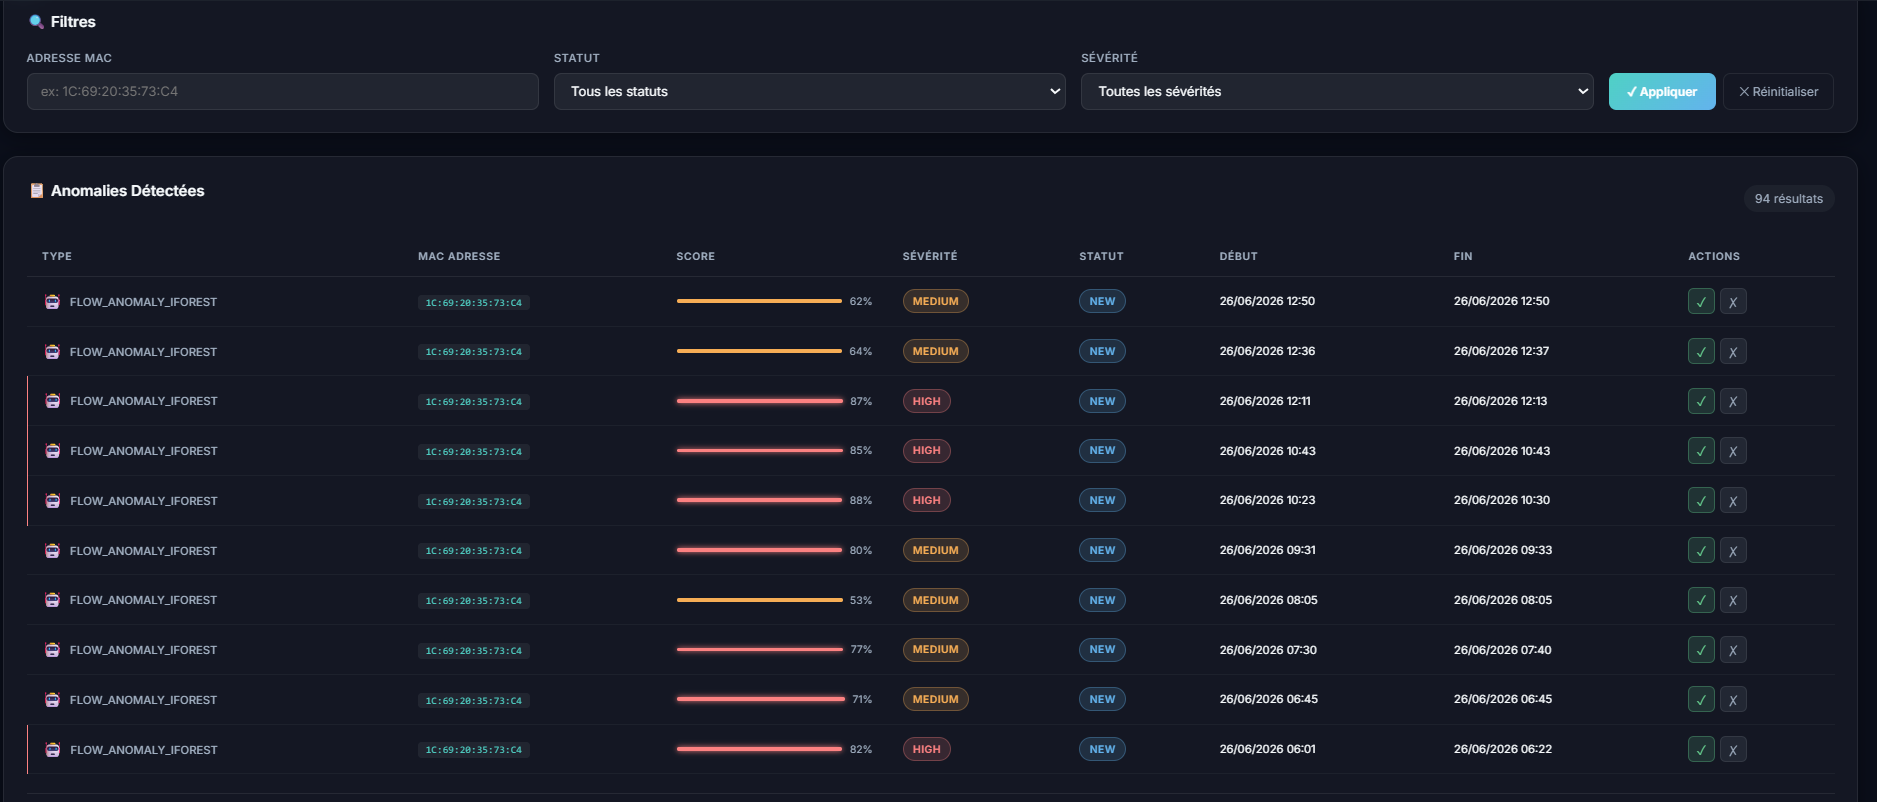
\includegraphics[width=\textwidth]{images/real.png}
    \caption{Écran principal du dashboard Droppy}
    \label{fig:dashboard}
\end{figure}


\subsection{Organisation de l'interface}

L'interface a été conçue afin de regrouper les informations essentielles dans
une présentation claire et directement exploitable par l'utilisateur.

\begin{figure}[H]
    \centering
    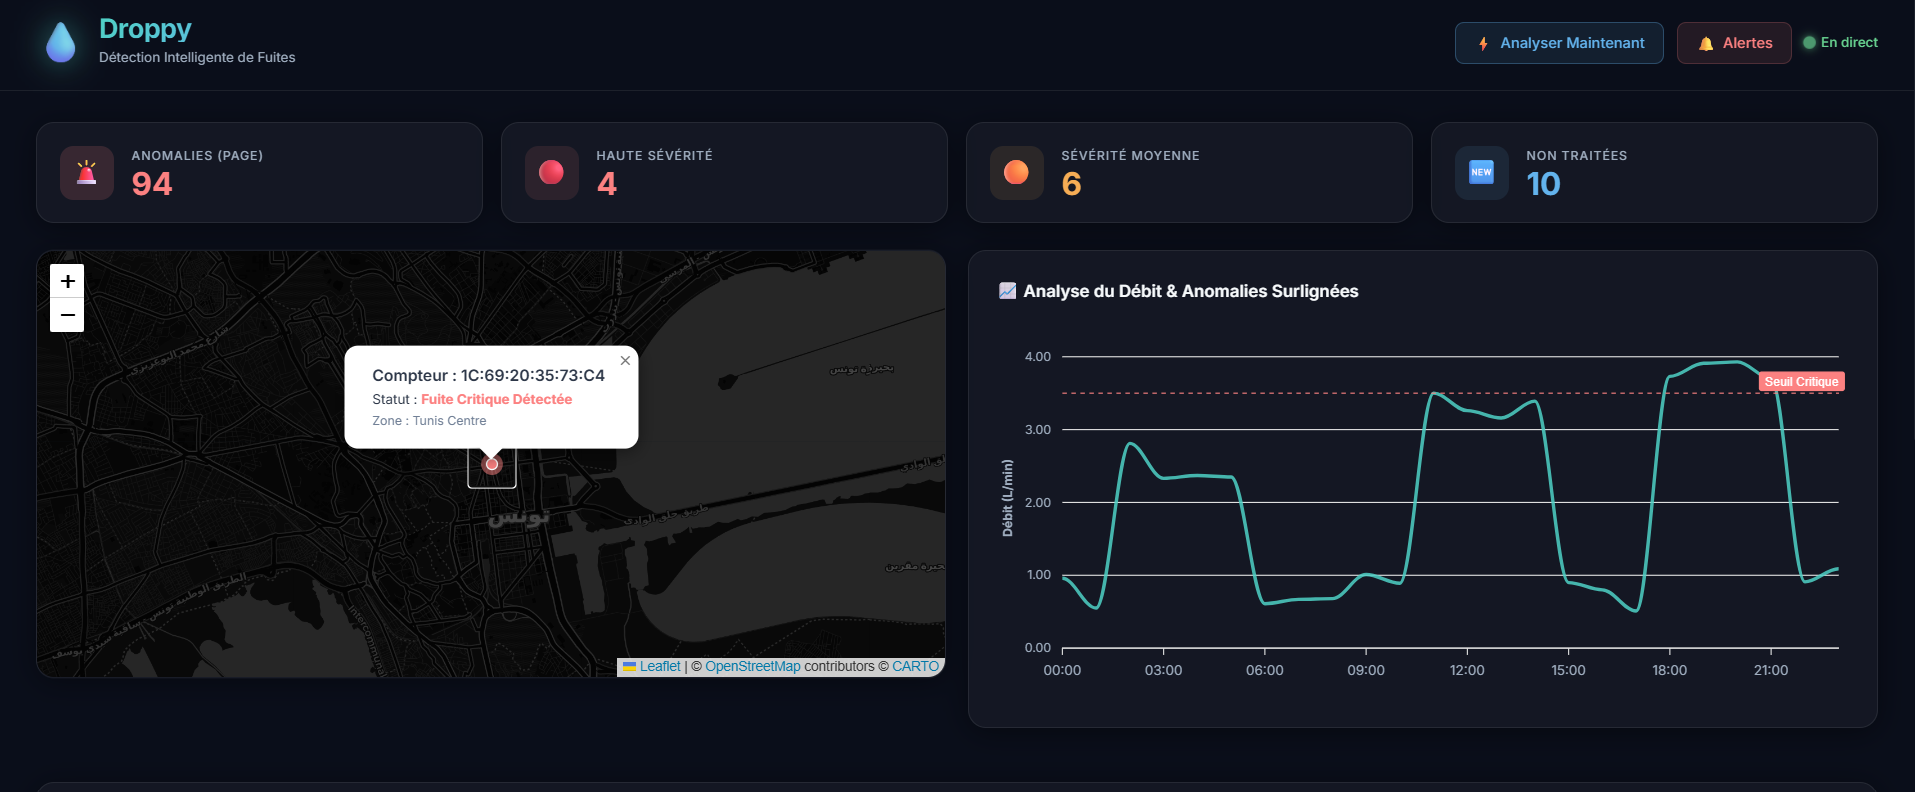
\includegraphics[width=\textwidth]{images/real2.png}
    \caption{Organisation générale de l'interface}
    \label{fig:interface-generale}
\end{figure}


% =============================================================================
% 4.3 SUPERVISION DES ANOMALIES
% =============================================================================

\section{Visualisation des données}

\subsection{Graphiques de suivi}

Les graphiques permettent de visualiser l'évolution des données et de
faciliter l'interprétation des différents événements observés.

\begin{figure}[H]
    \centering
    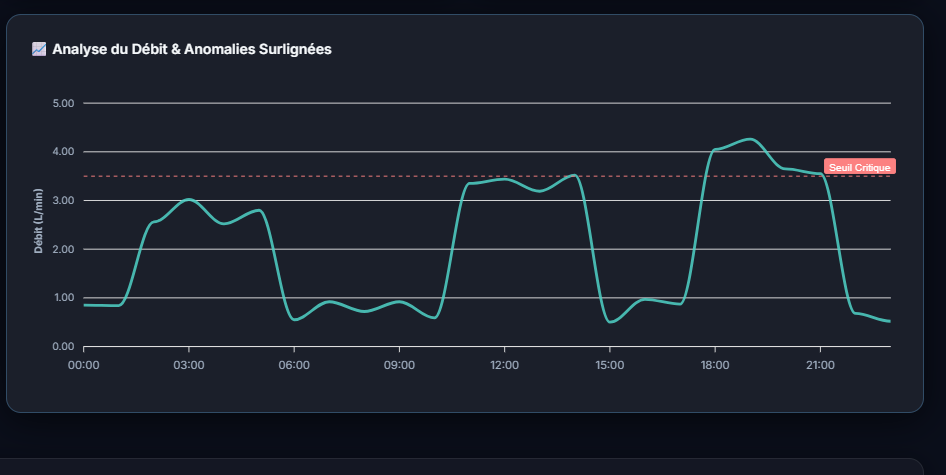
\includegraphics[width=\textwidth]{images/analyse.png}
    \caption{Visualisation graphique des données}
    \label{fig:graphiques}
\end{figure}



\subsection{Visualisation cartographique}

La carte permet de localiser les événements associés aux dispositifs
supervisés et d'offrir une représentation géographique des anomalies.

\begin{figure}[H]
    \centering
    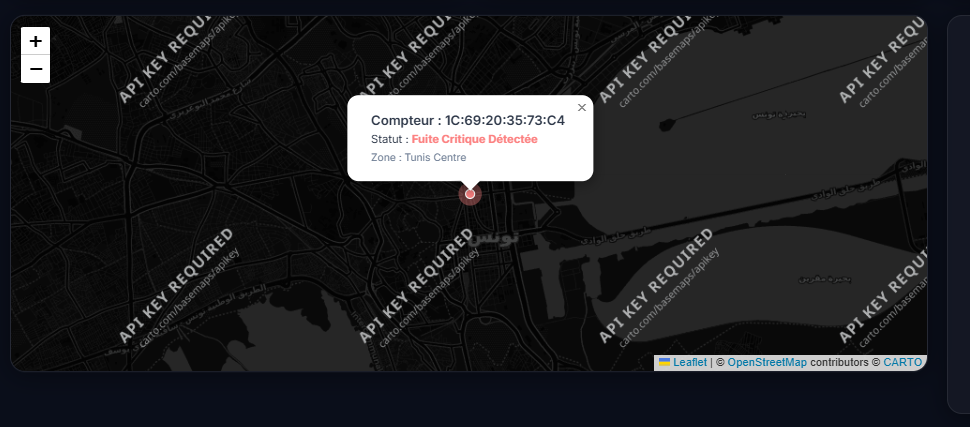
\includegraphics[width=\textwidth]{images/carteographie.png}
    \caption{Visualisation cartographique des anomalies}
    \label{fig:carte}
\end{figure}


% =============================================================================
% 4.5 ANALYSE INTELLIGENTE
% =============================================================================

\section{Analyse intelligente}
\subsection{Déclenchement d'une analyse}
L'utilisateur peut lancer une analyse depuis l'interface afin d'obtenir une
évaluation de l'état d'un dispositif.

\begin{figure}[H]
    \centering
    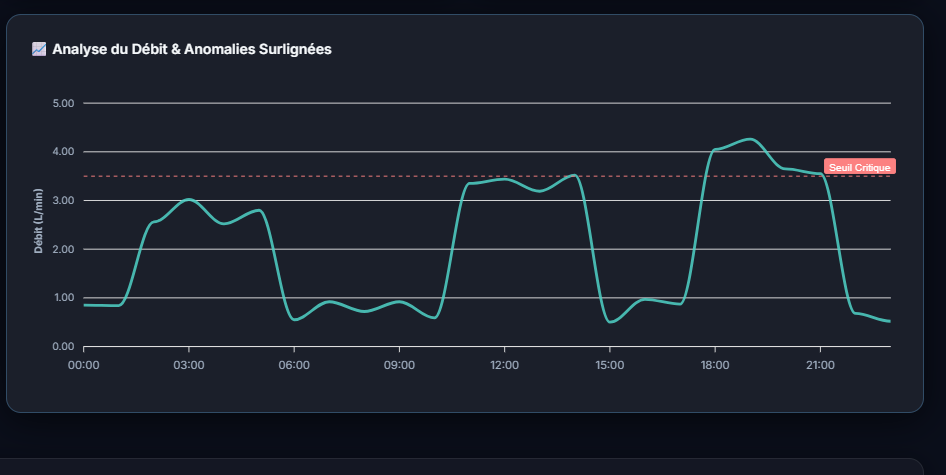
\includegraphics[width=\textwidth]{images/analyse.png}
    \caption{Déclenchement d'une analyse}
    \label{fig:analyse}
\end{figure}


\section{Conclusion}

Ce chapitre a présenté la réalisation de l'application Droppy à travers ses
principales interfaces et fonctionnalités.

Les différentes captures permettent d'illustrer concrètement le résultat
final de la solution, depuis la supervision générale jusqu'à la consultation
des anomalies, la visualisation des données, l'analyse et la prévision.

Le chapitre suivant sera consacré aux tests et à la validation de la solution.

% -----------------------------------------------------------------------------
% CHAPITRE 5
% -----------------------------------------------------------------------------

% =============================================================================
% CHAPITRE 5 — INTELLIGENCE ARTIFICIELLE ET DÉTECTION DES ANOMALIES
% =============================================================================

\chapter{Intelligence artificielle et détection des anomalies}

% =============================================================================
% 5.1 INTRODUCTION
% =============================================================================

\section{Introduction}

L'intelligence artificielle constitue l'un des éléments centraux de la
solution Droppy. Elle permet d'analyser automatiquement les données de
télémétrie afin d'identifier des comportements inhabituels et d'estimer
l'évolution future de la consommation.

L'approche retenue ne repose pas sur un unique mécanisme. Le service
d'intelligence artificielle combine des règles métier avec des méthodes
d'apprentissage automatique et de prévision. Cette combinaison permet
d'exploiter à la fois les connaissances liées au fonctionnement du réseau
et les comportements observés dans les données.

Le pipeline développé dans Droppy peut être résumé comme suit :

\begin{center}
\textbf{Données}
$\rightarrow$
\textbf{Nettoyage}
$\rightarrow$
\textbf{Prétraitement}
$\rightarrow$
\textbf{Détection}
$\rightarrow$
\textbf{Agrégation}
$\rightarrow$
\textbf{Résultat}
\end{center}


% =============================================================================
% 5.2 PIPELINE DE TRAITEMENT
% =============================================================================

\section{Pipeline de traitement des données}

Avant l'application des mécanismes de détection, les données sont chargées,
nettoyées puis préparées pour les différents traitements.

Le microservice IA sépare cette chaîne en plusieurs étapes correspondant au
chargement des mesures, au nettoyage et au prétraitement des données. Cette
organisation permet de disposer d'un flux de traitement homogène avant
l'exécution des différents mécanismes d'analyse.

\begin{figure}[H]
    \centering
    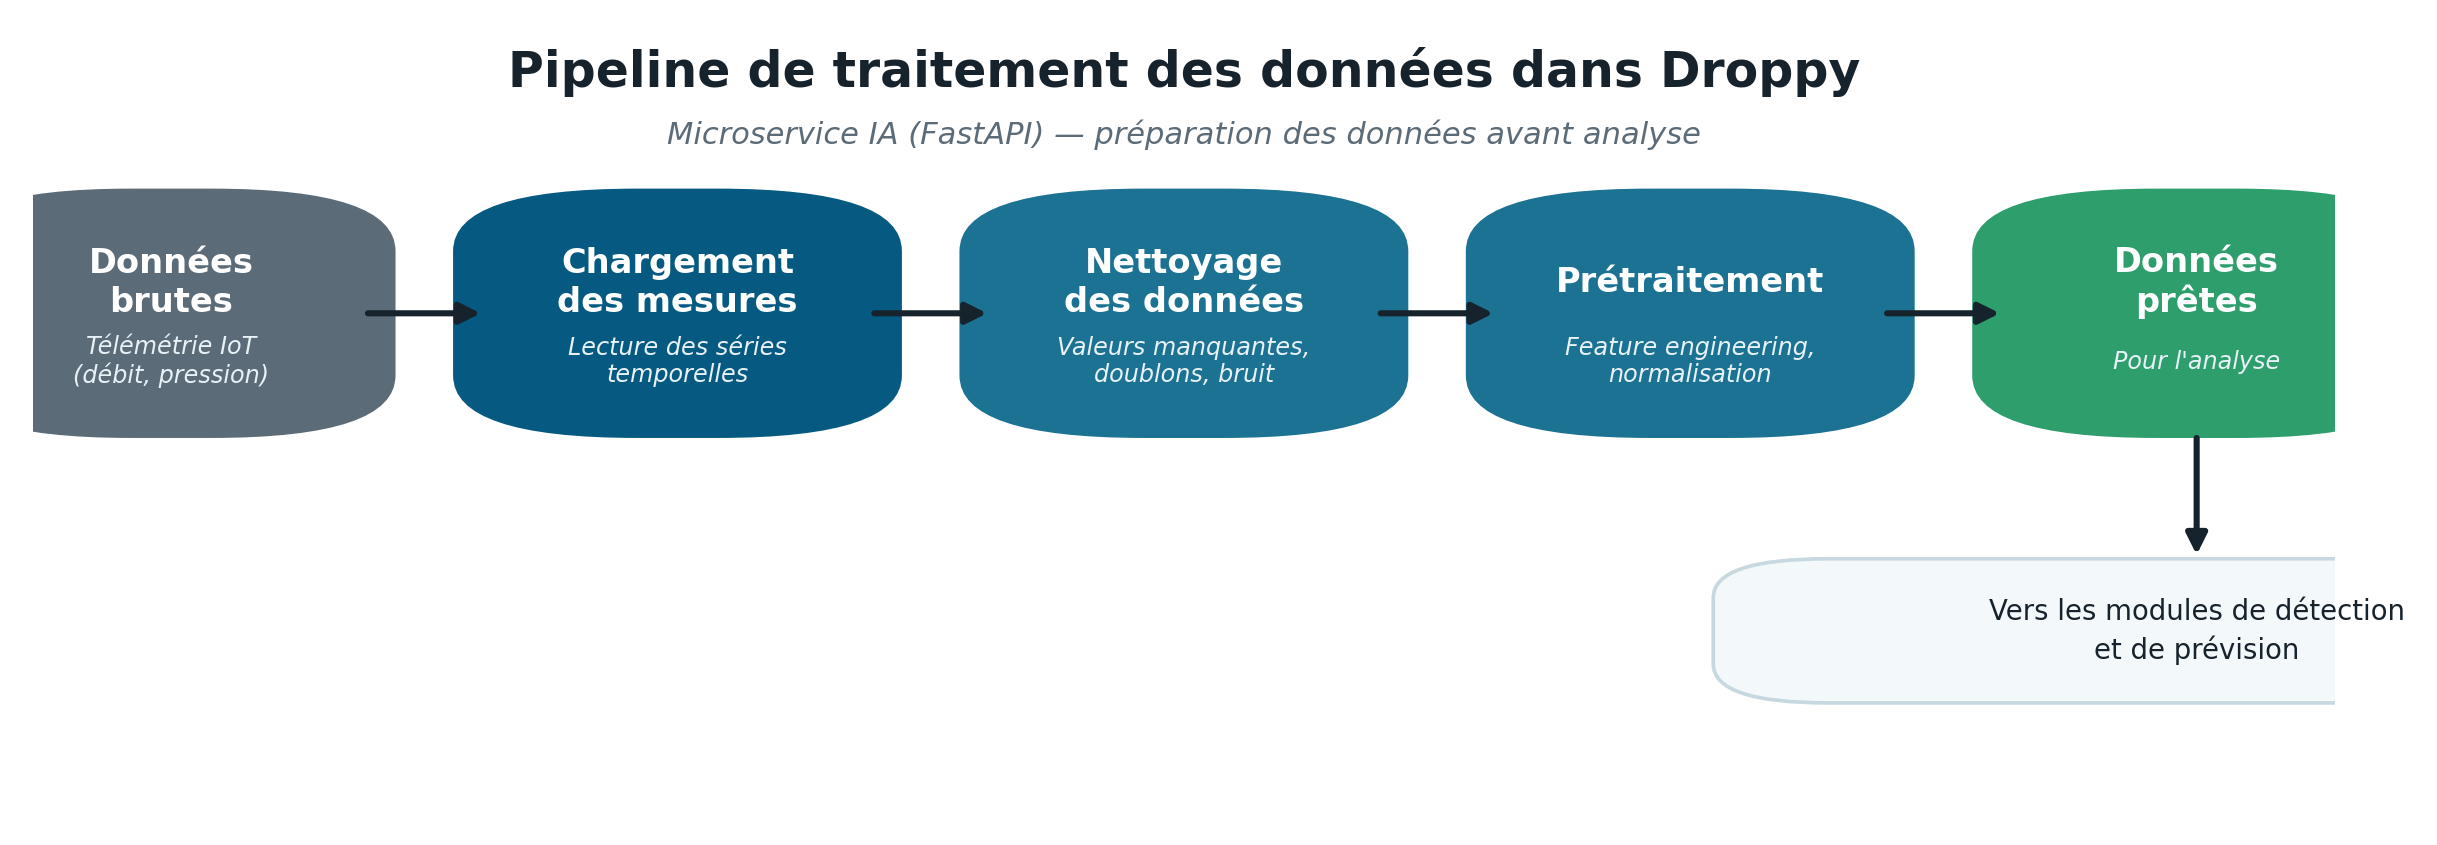
\includegraphics[width=0.90\textwidth]{images/pipeline-ia.png}
    \caption{Pipeline de traitement des données dans Droppy}
    \label{fig:pipeline-ia}
\end{figure}

Cette séparation permet également de réutiliser les mêmes étapes de
préparation pour les différents mécanismes d'analyse.


% =============================================================================
% 5.3 STRATÉGIE DE DÉTECTION
% =============================================================================

\section{Stratégie de détection des anomalies}

La détection mise en œuvre dans Droppy repose sur une approche hybride.
Lorsqu'une prédiction est demandée, le microservice exécute plusieurs
mécanismes indépendants puis regroupe leurs résultats.

Quatre sources de détection sont actuellement intégrées :

\begin{itemize}

    \item la détection du \textit{Minimum Night Flow} ;

    \item la détection d'incohérences liées aux vannes ;

    \item la détection statistique par \textit{Isolation Forest} ;

    \item la détection d'écarts de consommation à partir du modèle de
    prévision.

\end{itemize}

Les résultats sont ensuite regroupés et les événements correspondant au même
type et au même intervalle temporel sont dédoublonnés.

\begin{figure}[H]
    \centering
    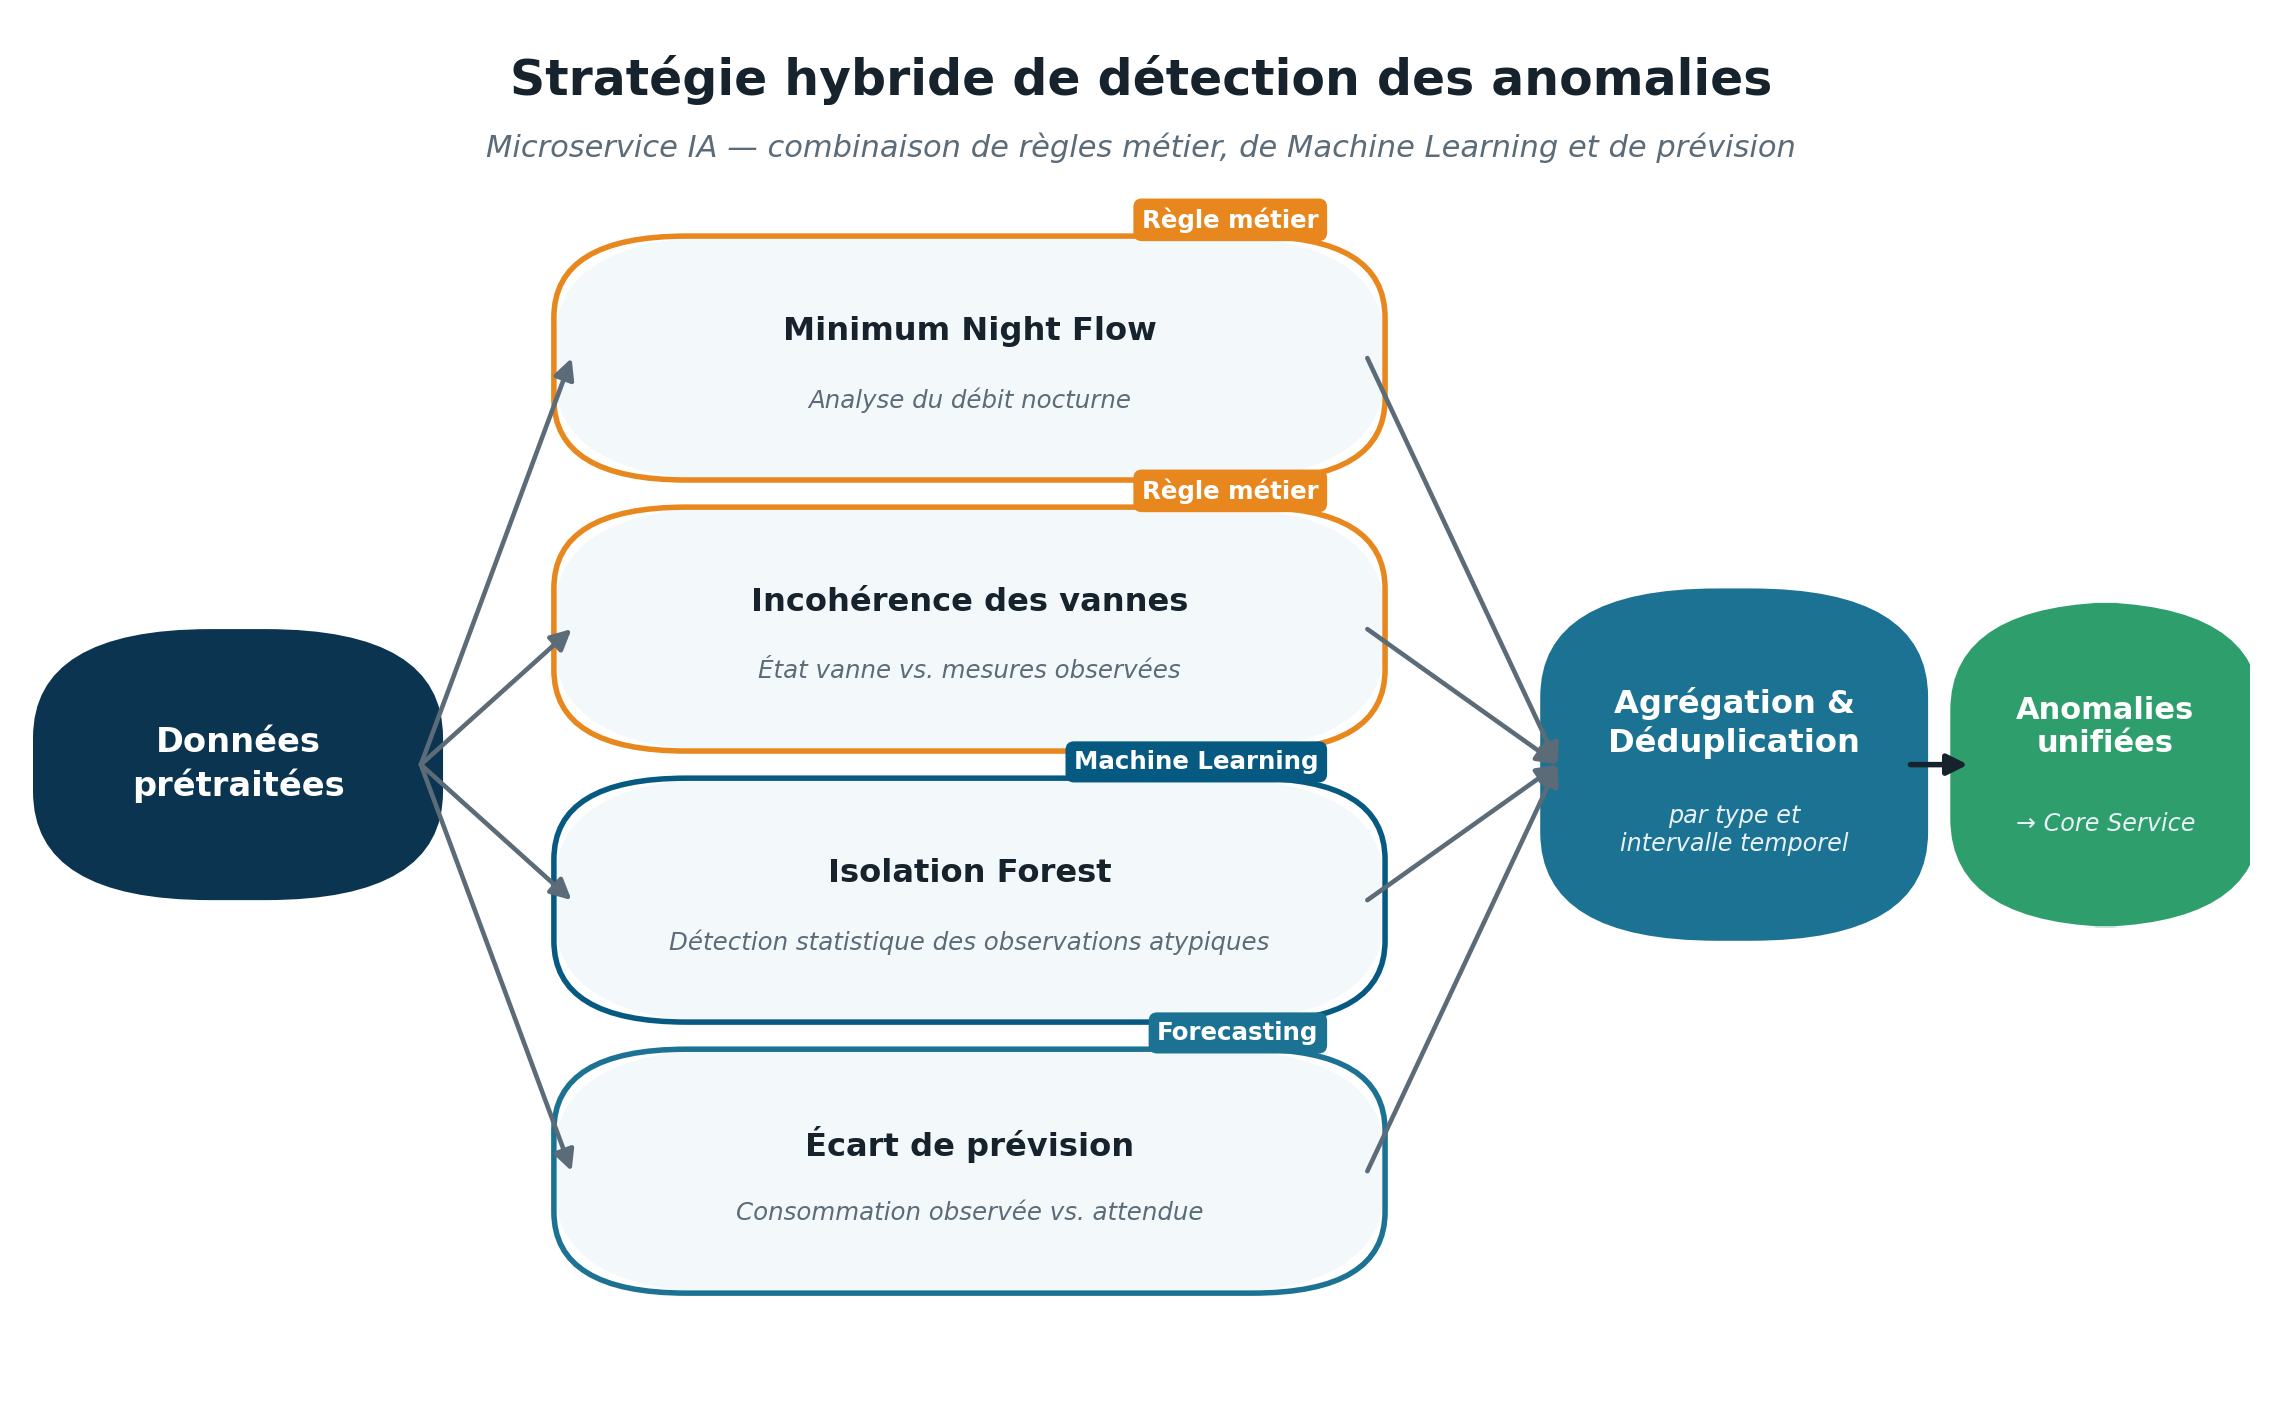
\includegraphics[width=0.90\textwidth]{images/strategie-detection.png}
    \caption{Stratégie hybride de détection des anomalies}
    \label{fig:strategie-detection}
\end{figure}


% =============================================================================
% 5.4 DÉTECTION PAR RÈGLES MÉTIER
% =============================================================================

\section{Détection basée sur les règles métier}

\subsection{Minimum Night Flow}

Le premier mécanisme repose sur l'analyse du débit pendant les périodes
nocturnes. L'objectif est d'identifier des situations dans lesquelles le
comportement observé s'écarte du fonctionnement attendu pendant ces
périodes.

Cette approche permet d'intégrer directement une connaissance métier dans
le processus de détection, sans dépendre exclusivement d'un modèle
d'apprentissage automatique.

\subsection{Incohérence liée aux vannes}

Le second mécanisme recherche des incohérences entre l'état d'une vanne et
le comportement observé dans les mesures.

Cette règle permet de détecter des situations dans lesquelles les mesures
observées ne correspondent pas au fonctionnement attendu du dispositif.


% =============================================================================
% 5.5 DÉTECTION PAR ISOLATION FOREST
% =============================================================================

\section{Détection par Isolation Forest}

En complément des règles métier, Droppy utilise l'algorithme
\textit{Isolation Forest} pour identifier automatiquement les observations
qui présentent un comportement inhabituel.

Contrairement à une classification supervisée classique, cette méthode est
adaptée à la détection d'observations atypiques. Le modèle est entraîné à
partir des données préparées puis utilisé lors de l'analyse d'un dispositif.

Dans l'implémentation de Droppy, le modèle est chargé pour le dispositif
concerné et appliqué aux données prétraitées. Le résultat produit contribue
ensuite à la liste globale des anomalies.

\begin{figure}[H]
    \centering
    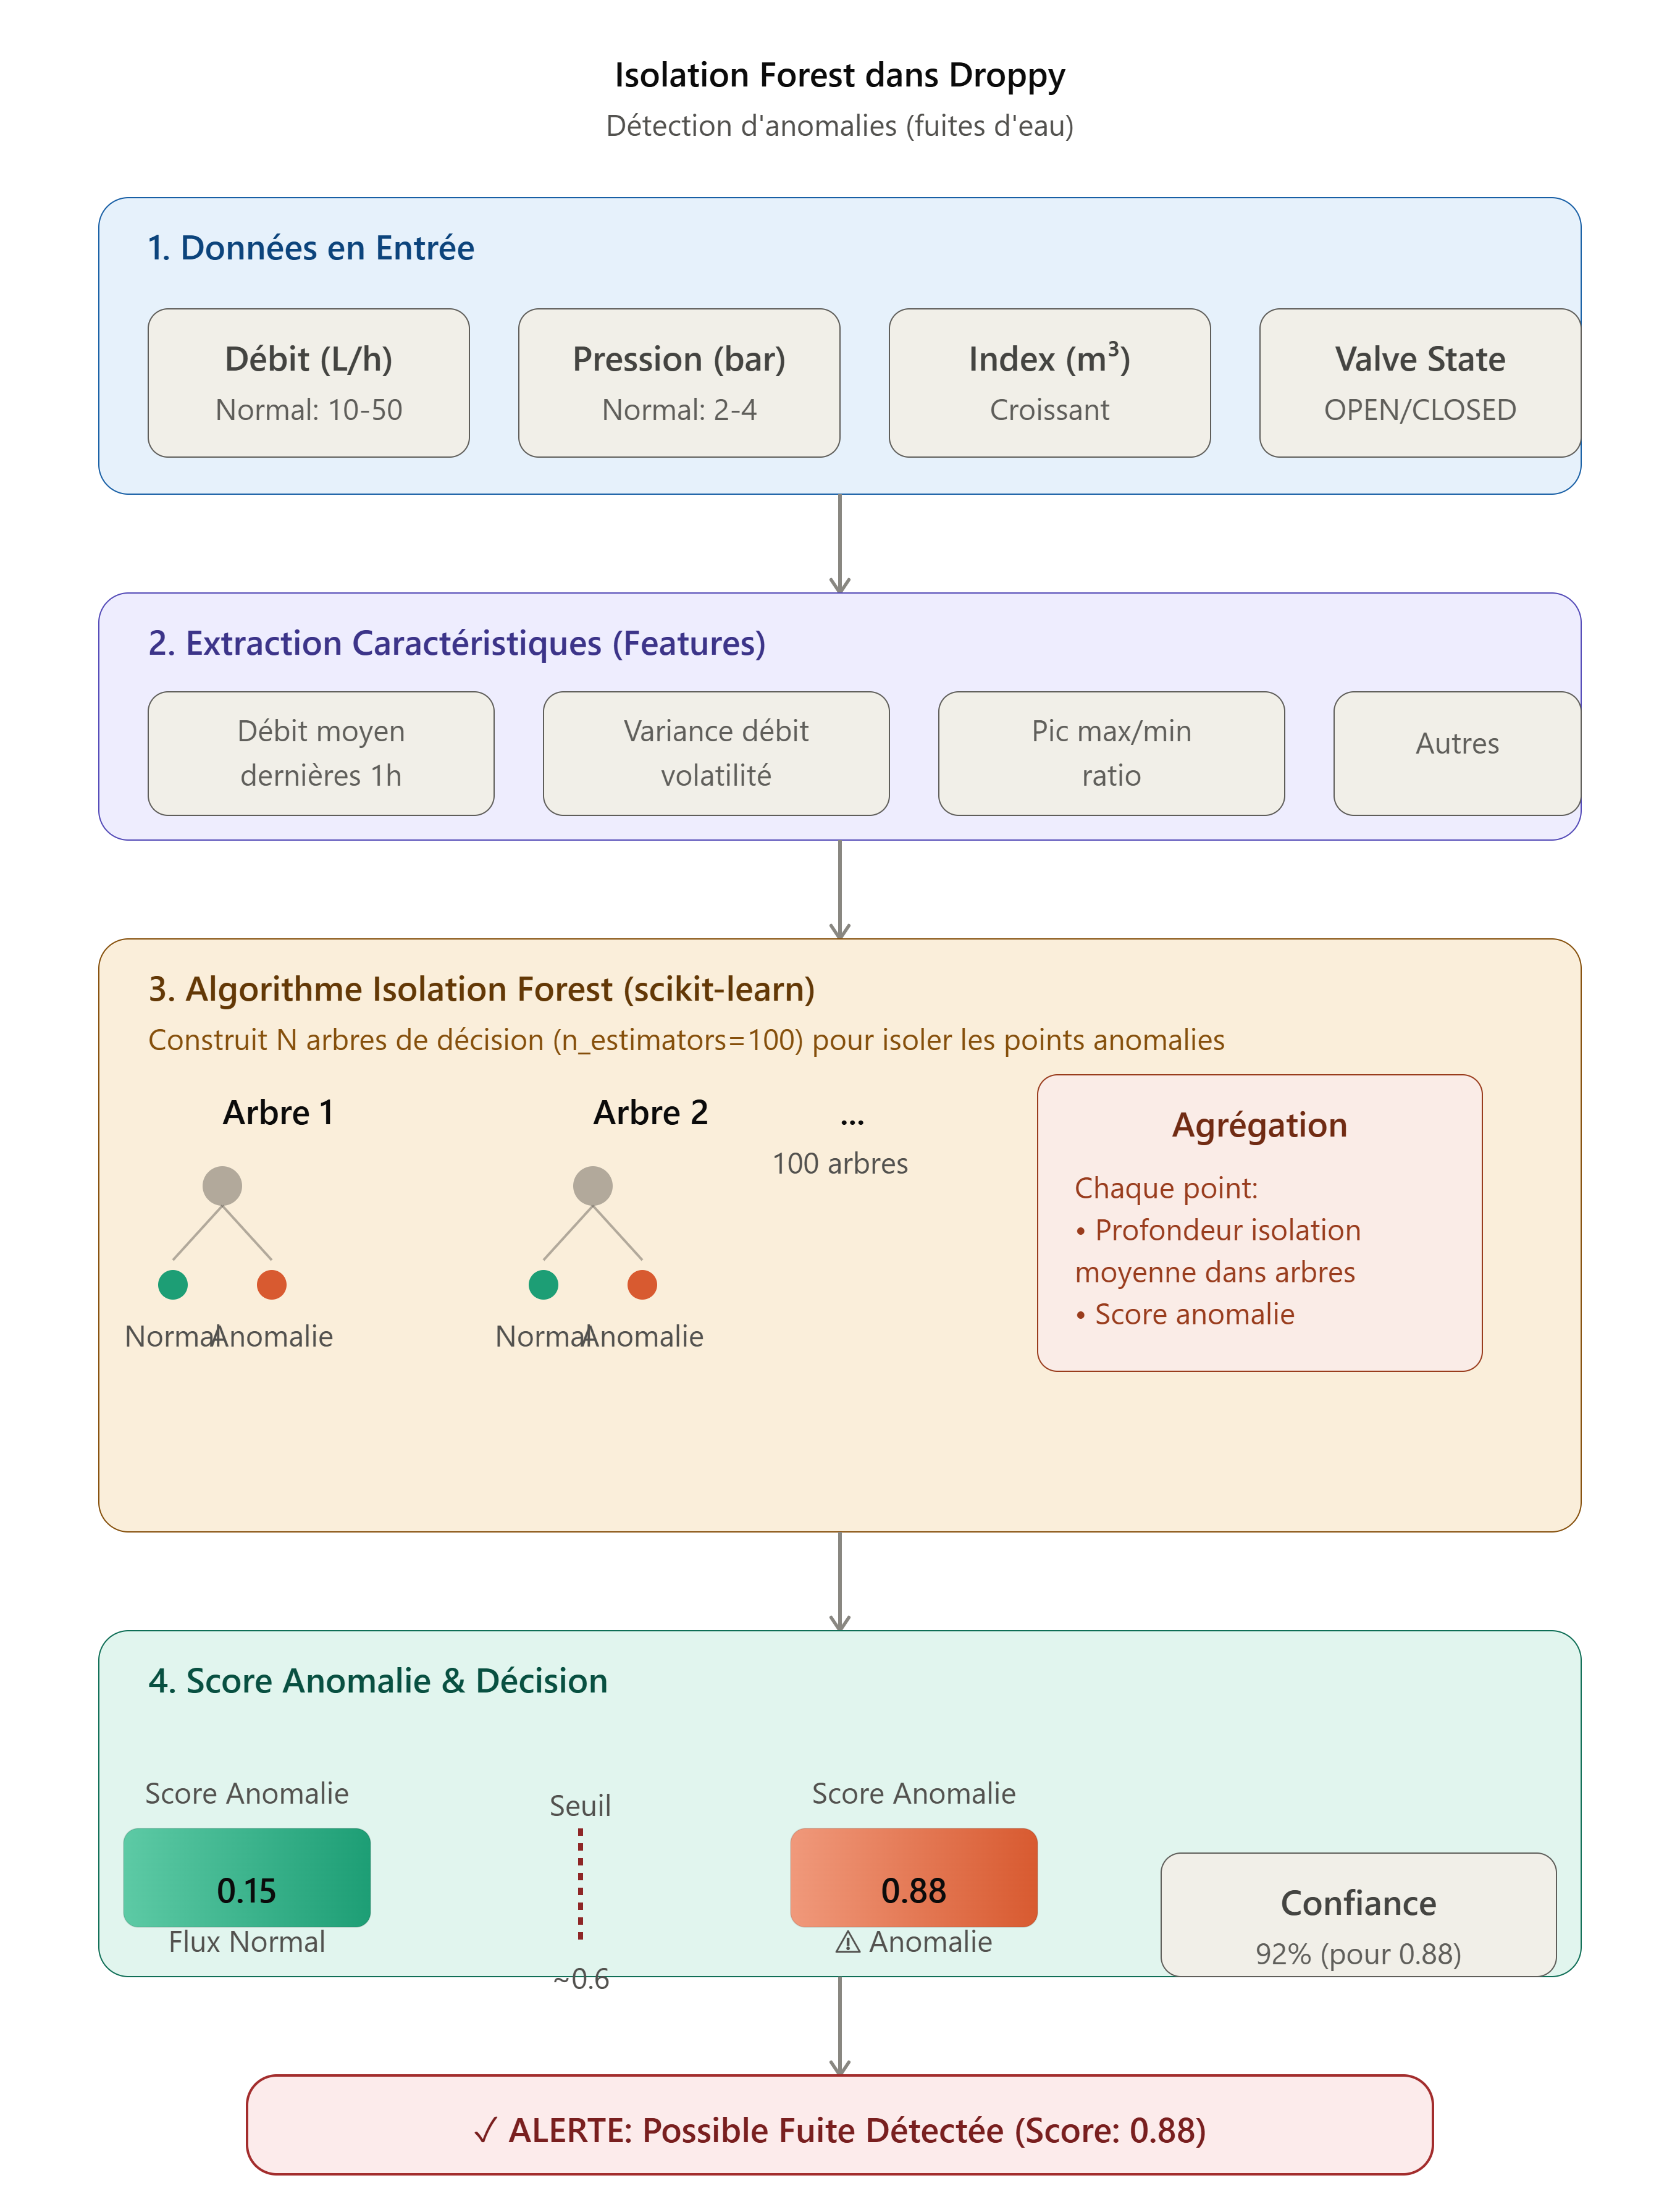
\includegraphics[width=0.85\textwidth]{images/isolation_forest_droppy_principle.png}
    \caption{Principe d'utilisation de l'Isolation Forest dans Droppy}
    \label{fig:isolation-forest}
\end{figure}


% =============================================================================
% 5.6 PRÉVISION DE CONSOMMATION
% =============================================================================

\section{Agrégation des résultats}

L'une des caractéristiques importantes de l'approche adoptée est la
combinaison des différentes sources de détection.

Pour une même période d'analyse, les résultats issus des règles métier,
de l'Isolation Forest et de l'analyse de déviation de consommation sont
regroupés dans une même réponse.

Le système applique ensuite une étape de déduplication afin d'éviter de
retourner plusieurs fois un même événement lorsqu'il est identifié par
plusieurs mécanismes.

Cette stratégie permet de produire une sortie unifiée destinée au Core
Service et, finalement, au dashboard Droppy.


% =============================================================================
% 5.9 RÉSULTAT DE L'ANALYSE
% =============================================================================

\section{Résultat de l'analyse}

Chaque anomalie produite par le microservice contient plusieurs informations
permettant son exploitation par les composants du système.

Le résultat de prédiction comprend notamment :

\begin{itemize}

    \item le type de l'anomalie ;

    \item le score associé à la détection ;

    \item l'intervalle temporel concerné ;

    \item le niveau de sévérité.

\end{itemize}

Ces informations sont ensuite transmises au Core Service afin d'être
intégrées dans le système de supervision.


% =============================================================================
% 5.10 API DU SERVICE INTELLIGENT
% =============================================================================

\section{Exposition des fonctionnalités IA}

Les fonctionnalités d'intelligence artificielle sont exposées à travers le
microservice FastAPI.

Trois opérations principales sont proposées :

\begin{itemize}

    \item \texttt{/train/\{mac\}} : entraînement ou réentraînement des
    modèles associés à un dispositif ;

    \item \texttt{/predict/\{mac\}} : exécution de la détection combinant
    les différents mécanismes d'analyse ;

    \item \texttt{/forecast/\{mac\}} : génération des prévisions de
    consommation.

\end{itemize}

Cette séparation permet au Core Service de solliciter indépendamment les
opérations d'entraînement, de détection et de prévision.


% =============================================================================
% 5.11 SYNTHÈSE
% =============================================================================

\section{Synthèse}

L'intelligence de Droppy repose ainsi sur une combinaison de plusieurs
mécanismes complémentaires.

Les règles métier permettent d'intégrer les connaissances liées au
fonctionnement du réseau, tandis que l'Isolation Forest apporte une capacité
de détection automatique des comportements atypiques. Le modèle de prévision
complète cette approche en permettant à la fois d'estimer la consommation
future et d'identifier des écarts par rapport au comportement attendu.

Cette approche hybride constitue le cœur analytique de Droppy et permet de
transformer les données de télémétrie en événements exploitables par la
plateforme de supervision.


% =============================================================================
% 5.12 CONCLUSION
% =============================================================================

\section{Conclusion}

Ce chapitre a présenté le fonctionnement de la composante d'intelligence
artificielle de Droppy.

La solution combine un pipeline de préparation des données, des règles
métier, l'algorithme Isolation Forest et un mécanisme de prévision de
consommation. Les résultats issus de ces différents traitements sont
agrégés afin de produire une vision unifiée des anomalies détectées.

Le chapitre suivant sera consacré aux tests et à la validation de la solution
afin d'évaluer le comportement des différents composants et les résultats
obtenus.

% -----------------------------------------------------------------------------
% CHAPITRE 6
% -----------------------------------------------------------------------------

% =============================================================================
% CHAPITRE 6 — CONCLUSION GÉNÉRALE ET PERSPECTIVES
% =============================================================================

\chapter{Conclusion générale et perspectives}

% =============================================================================
% 6.1 CONCLUSION GÉNÉRALE
% =============================================================================

\section{Conclusion générale}

Ce projet de stage a porté sur la conception et la réalisation de Droppy,
une solution intelligente dédiée à la supervision et à l'analyse des données
issues d'un réseau d'eau.

L'objectif principal était de proposer une plateforme capable d'exploiter
les données de télémétrie afin d'identifier automatiquement des comportements
anormaux et de fournir des informations utiles à la supervision du réseau.

La réalisation du projet a permis de mettre en place une architecture
distribuée intégrant une interface de supervision, un service central
d'orchestration et un microservice dédié aux traitements d'intelligence
artificielle. Cette organisation a permis de séparer les différentes
responsabilités tout en assurant leur communication.

La conception de la solution a été formalisée à travers plusieurs modèles
UML permettant de représenter les interactions, l'architecture, les
séquences principales, la structure des classes et l'organisation du
déploiement.

La réalisation de l'application a ensuite permis de concrétiser ces choix
à travers un dashboard destiné à la supervision des anomalies, à la
visualisation des données et à la consultation des prévisions.

La composante intelligente constitue également un élément essentiel de
Droppy. L'approche retenue combine plusieurs mécanismes complémentaires,
notamment des règles métier, l'Isolation Forest et la prévision de
consommation. Cette combinaison permet d'obtenir une analyse plus adaptée
aux caractéristiques des données étudiées.

Ainsi, ce projet a permis de mettre en pratique différentes compétences
liées au développement logiciel, à la conception d'architectures
distribuées, au traitement des données et à l'intelligence artificielle,
tout en répondant à une problématique concrète de supervision.


% =============================================================================
% 6.2 APPORTS DU PROJET
% =============================================================================

\section{Apports du projet}

La réalisation de Droppy a permis d'aboutir à une solution intégrant
plusieurs fonctionnalités complémentaires :

\begin{itemize}

    \item supervision des anomalies détectées ;

    \item visualisation des informations à travers un dashboard ;

    \item analyse automatique des comportements inhabituels ;

    \item génération de prévisions de consommation ;

    \item transmission des événements en temps réel ;

    \item centralisation des résultats pour leur exploitation par
    l'utilisateur.

\end{itemize}

Au-delà des fonctionnalités développées, ce projet a également constitué une
expérience permettant de mieux comprendre les contraintes liées à
l'intégration de plusieurs services logiciels au sein d'une même solution.


% =============================================================================
% 6.3 LIMITES DE LA SOLUTION
% =============================================================================

\section{Limites de la solution}

Malgré les fonctionnalités réalisées, certaines améliorations restent
possibles.

Les performances des mécanismes de détection dépendent notamment de la
qualité et de la disponibilité des données historiques. La diversité des
comportements observés sur différents dispositifs peut également nécessiter
une adaptation des modèles et des paramètres utilisés.

Par ailleurs, l'évolution de la solution vers un environnement de production
à grande échelle nécessiterait de renforcer certains aspects liés au
déploiement, à la supervision des services et à la gestion d'un nombre plus
important de dispositifs.


% =============================================================================
% 6.4 PERSPECTIVES
% =============================================================================

\section{Perspectives}

Plusieurs évolutions peuvent être envisagées afin d'améliorer les capacités
de Droppy.

\subsection{Amélioration des modèles d'intelligence artificielle}

Une première perspective consiste à enrichir les modèles d'analyse en
utilisant davantage de données historiques et en expérimentant différentes
approches d'apprentissage automatique afin d'améliorer la détection des
comportements atypiques.

\subsection{Extension de la supervision}

La solution pourrait être étendue afin de prendre en charge un nombre plus
important de dispositifs et de réseaux. Une gestion plus avancée des
dispositifs permettrait également d'adapter les analyses aux caractéristiques
de chaque installation.

\subsection{Amélioration du système d'alertes}

Le système de supervision pourrait être complété par différents canaux
d'alerte afin de permettre une notification plus rapide des événements
importants.

\subsection{Déploiement dans un environnement Cloud}

Une évolution vers une infrastructure Cloud permettrait de faciliter le
déploiement, la disponibilité et la montée en charge de la solution.

\subsection{Développement d'une application mobile}

Une application mobile pourrait également être développée afin de permettre
aux opérateurs de consulter les anomalies et les alertes depuis leurs
appareils mobiles.

\subsection{Évolution vers une maintenance prédictive}

À plus long terme, les données historiques et les résultats des modèles
pourraient être exploités afin d'aller au-delà de la simple détection
d'anomalies et de proposer une approche de maintenance prédictive.


% =============================================================================
% 6.5 CONCLUSION FINALE
% =============================================================================

\section{Conclusion finale}

Le développement de Droppy a permis de mettre en œuvre une solution complète
associant supervision, analyse de données, intelligence artificielle et
visualisation.

Le projet constitue une première base pour une plateforme pouvant évoluer
vers une supervision plus automatisée et plus prédictive des réseaux d'eau.

Les perspectives identifiées offrent ainsi plusieurs possibilités
d'évolution, aussi bien sur le plan fonctionnel que sur le plan technique.
Elles permettraient notamment d'améliorer la précision des analyses,
d'étendre la solution à davantage de dispositifs et de faciliter son
exploitation dans un environnement réel à grande échelle.

% =============================================================================
% BIBLIOGRAPHIE
% =============================================================================

\begin{thebibliography}{9}

\addcontentsline{toc}{chapter}{Bibliographie}

\bibitem{sklearn}

Pedregosa, F. et al. (2011).

\textit{Scikit-learn: Machine Learning in Python}.

Journal of Machine Learning Research,
12, pp. 2825--2830.

\bibitem{liu2008}

Liu, F. T., Ting, K. M. et Zhou, Z.-H. (2008).

\textit{Isolation Forest}.

Proceedings of the 2008 IEEE International Conference on
Data Mining (ICDM).

\bibitem{fastapi}

Ramírez, S.

\textit{FastAPI Documentation}.

\url{https://fastapi.tiangolo.com/}

\bibitem{spring}

VMware.

\textit{Spring Boot Reference Documentation}.

\url{https://spring.io/projects/spring-boot}

\bibitem{angular}

Google.

\textit{Angular Documentation}.

\url{https://angular.dev/}

\bibitem{mnf}

International Water Association.

\textit{Minimum Night Flow for Leak Detection}.

Best Practice Guidelines.

\bibitem{sfm}

Groupe SFM.

\textit{SFM Connect -- Solutions IoT Énergie \& Eau}.

\url{https://linkedin.com/company/groupe-sfm}

\end{thebibliography}

% =============================================================================
% ANNEXES
% =============================================================================

\appendix

\chapter{Annexes}

\section{User Stories implémentées}

\begin{table}[H]
  \centering
  \caption{Correspondance User Stories / modules}
  \begin{tabular}{lll}
    \toprule
    \textbf{US} & \textbf{Description} & \textbf{Module} \\
    \midrule
    US-05 & Health check & FastAPI \\
    US-06 & Connexion SQLAlchemy & loader.py \\
    US-07 & Prétraitement & preprocessor.py \\
    US-08 & Minimum Night Flow & mnf.py \\
    US-09 & Isolation Forest & isolation\_forest.py \\
    US-10 & Valve Inconsistency & valve\_inconsistency.py \\
    US-11 & Prédiction agrégée & main.py \\
    US-12 & Prévision consommation & forecaster.py \\
    \bottomrule
  \end{tabular}
\end{table}

\section{Configuration de déploiement}

\begin{table}[H]
  \centering
  \caption{Services et ports}
  \begin{tabular}{lll}
    \toprule
    \textbf{Service} & \textbf{Port} & \textbf{Commande} \\
    \midrule
    FastAPI & 8001 & \texttt{uvicorn src.main:app --port 8001} \\
    Spring Boot & 8082 & \texttt{mvn spring-boot:run} \\
    Angular & 4200 & \texttt{ng serve --port 4200} \\
    \bottomrule
  \end{tabular}
\end{table}

\section{Structure du projet source}

\begin{lstlisting}[caption={Arborescence du projet Droppy}, label={lst:structure}]
stage/
|-- core-service/          # Spring Boot Backend
|   |-- src/main/java/     # Controllers, Services, Models
|   |-- pom.xml
|   `-- db/changelog/      # Liquibase
|-- dashboard-angular/     # Angular 19 UI
|   |-- src/app/components/
|   |-- src/app/services/
|   `-- package.json
|-- src/                   # FastAPI AI Engine
|   |-- data/              # loader, cleaner
|   |-- features/          # preprocessor
|   |-- models/            # ML detectors
|   `-- main.py
|-- tests/                 # pytest
|-- models/                # Joblib serialized models
|-- requirements.txt
`-- run_app.bat
\end{lstlisting}


% =============================================================================
% FIN DU DOCUMENT
% =============================================================================

\end{document}